In this chapter, the results of the experiments performed to validate and test the methods presented in Chapter \ref{chap:methods} are discussed with the aim to establish the best model architecture. In order to do so, it is first necessary to briefly introduce the experimental setup on which this model comparison is conducted. \\
Each model is evaluated under two different regimes: \textit{Multi-Speaker} and \textit{Single-Speaker}. The former task aims to develop a system able to generalize the artificial \gls{bwe} to both female and male speakers with different accents. The latter one, as the name suggests, takes into account only data coming from a single speaker. Specifically for our experiments, the first speaker of the \gls{vctk} dataset. Both tasks are addressed in the reference papers too (\cite{lim2018time}, \cite{birnbaum2019temporal}). \\
As for software tools, the whole project is written in Python. This programming language is well suited to achieve the desired development purposes, since it offers a diverse set of tools for both \gls{dsp} and \gls{dl} applications. The main packages used in this work include Tensorflow, Scipy and Librosa. \\
%As motivated in the previous chapter, it is worth noting that this project requires large computational resources that arise from both the dataset size and the models' number of parameters. \\
We use Google Colaboratory (Colab), a cloud-based service accessible through a web browser. The key advantage of this environment is that it provides up to 25GB of RAM, and a free access to the high-end GPUs. This helps in reducing the computational time as GPUs are very powerful for massively parallel computations, such as the ones required for tensors (signals' data structure) processing.

\begin{figure}[H]
	\begin{subfigure}{.25\textwidth}
		\centering
		
\includegraphics[width=.7\linewidth]{img/colab_logo.png}
		\label{fig:colab_logo}
	\end{subfigure}%
	\begin{subfigure}{.25\textwidth}
		\centering
		
\includegraphics[width=.6\linewidth]{img/tensorflow_logo.png}
		\label{fig:tensorflow_logo}
	\end{subfigure}%
	\begin{subfigure}{.25\textwidth}
		\centering
		
\includegraphics[width=1.1\linewidth]{img/librosa_logo.png}
		\label{fig:librosa_logo}
	\end{subfigure}%
	\begin{subfigure}{.25\textwidth}
		\centering
		
\includegraphics[width=.55\linewidth]{img/scipy_logo.png}
		\label{fig:scipy_logo}
	\end{subfigure}
	\caption{From the left, the logos of Colab, Tensorflow, Librosa and Scipy.}
	\label{fig:fig}
\end{figure}

\section{Experimental Setup}
This paragraph aims to provide a clear specification of the experimental setup. A full description of the dataset and its preparation is provided along with the metrics used to evaluate the models. 

\subsection{Dataset and preparation}
Experiments reported in this thesis are undertaken using the most popular dataset for the audio SR task, i.e. \gls{vctk} \cite{yamagishi2019cstr}. In recent years, many researchers have used it (see e.g., \cite{birnbaum2019temporal}, \cite{lim2018time}, \cite{eskimez2019speech}, \cite{wang2018speech}), to such an extent that we can now consider this dataset as a benchmark for the \gls{bwe} problem. \\
This \gls{vctk} Corpus contains approximately 44 hours of speech data uttered by 109 English speakers, each of whom reads out about 400 different sentences. The dataset was initially designed for training Text-to-Speech synthesis systems. In fact, each recording is associated with the corresponding textual transcription. This data are used in this work in order to evaluate models' performance over the \gls{stt} task, whose details are discussed in section \ref{eval_methods}. \\
The \gls{vctk} Corpus encompasses speakers with various accents, as shown in Figure \ref{fig:accents_speakers}. \\
\begin{figure}[!htb]
	\begin{center}
		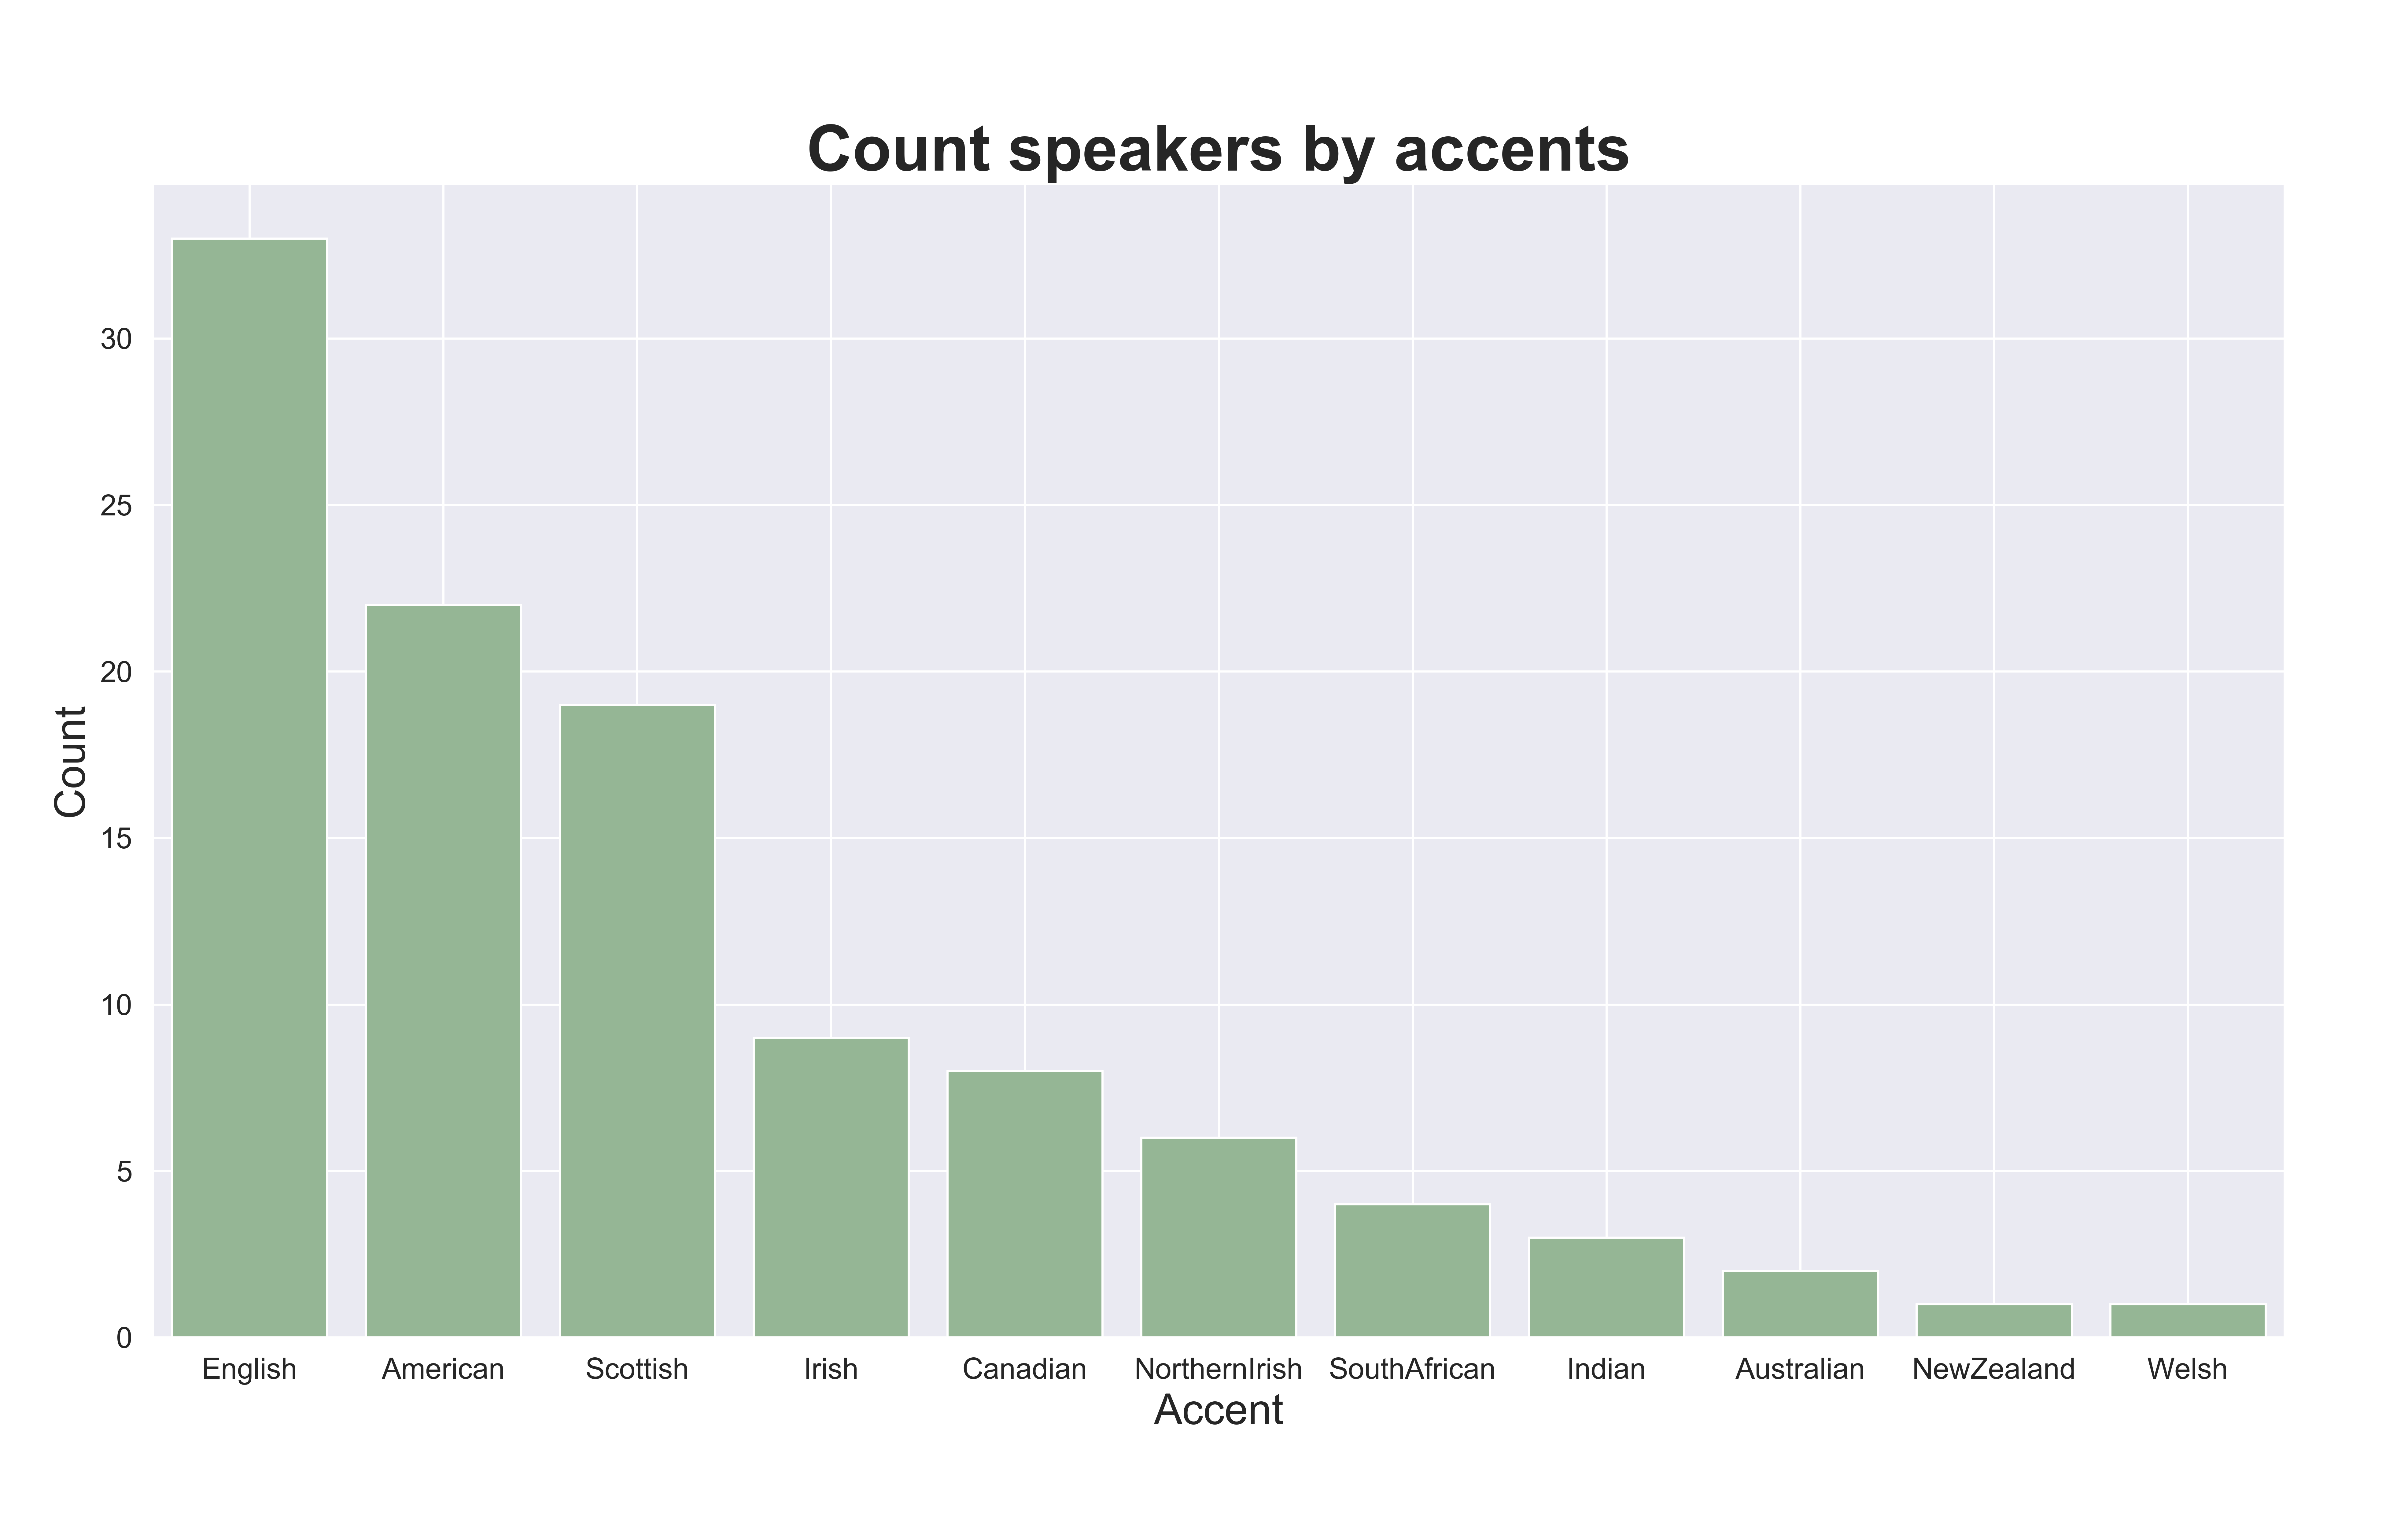
\includegraphics[scale=0.4]{img/count_speakers_by_accents.png}
		\caption{Bar chart showing the count of speakers in \gls{vctk} dataset based on their accent.}
		\label{fig:accents_speakers}
	\end{center}
\end{figure}
\noindent All speech data are clean, and they were originally recorded using an identical recording setup, i.e. 96 kHz sampling frequency at 24 bits in the same room, with the same microphone. All recordings were finally converted into 16 bits and downsampled to 48 kHz; this is the quality of data available online. \\
All recordings are further downsampled to 16 kHz for this project: it is possible to consider this sampling rate as $R_2$, i.e. the one that defines the ground truth $y = (y_{1/R_2}, y_{2/R_2}, \dots, y_{R_2S/R_2})$. It follows that, for a scaling ratio of $4 \times$, $R_1$ is equal to 4 kHz. It is noticeable that 16 kHz can be reasonably considered as a high quality standard for speech processing applications \cite{steidl2009automatic}; suffice to say that a standard telephone audio has a sampling rate of 8 kHz and 16-bit precision \cite{kamath2019automatic}. \\
As previously motivated, computational resources for this project are limited: in the multi-speaker task, it is not possible to use the whole dataset, as both reference papers, i.e. \cite{lim2018time} and \cite{birnbaum2019temporal}, do. In particular, authors of the reference papers train the models for this task on the first 100 \gls{vctk} speakers and test on the 9 remaining ones. We re-train their models, and the proposed system, on a sample of 40 speakers. However, the test set used in this project remains the same as the one used in both articles. By doing so, the comparison with newly developed models is placed in a fair context. Furthermore, the difference between the performance ~-~ of \gls{tfnet} and \gls{tfilm} ~-~ obtained in the original works and those obtained in this project, can be used to measure the negative impact that a drastic reduction in the dimensionality of the problem inevitably has on the performance of the system. \\
In addition, we also make use of a validation set, the importance of which is explained in section \ref{training_details}. It is important to highlight that there is no speaker overlap between train, validation and test partitions. This setting is selected in order to reduce performance over-estimation due to potential auto-correlations among different observations pertaining to the same speaker. \\
Both train and validation sets are sampled in a principled way: the main goal of this sample design is to maximize the model robustness with respect to the main factors of variation. When analyzing a speech recording, important factors concern, for example, the speaker’s sex and their accent. Thus, speakers are selected in order to ensure a balanced distribution by gender and a heterogeneous distribution of accents. From a theoretical point of view, this should encourage the creation of a \gls{dl} model that is robust with respect to variations of accent and gender. \\
The sampling performed also reflects the age distribution of the original dataset (especially for the female gender), as can be seen from Figure \ref{fig:age_dataset}. \\
\begin{figure}[H]
	\begin{center}
		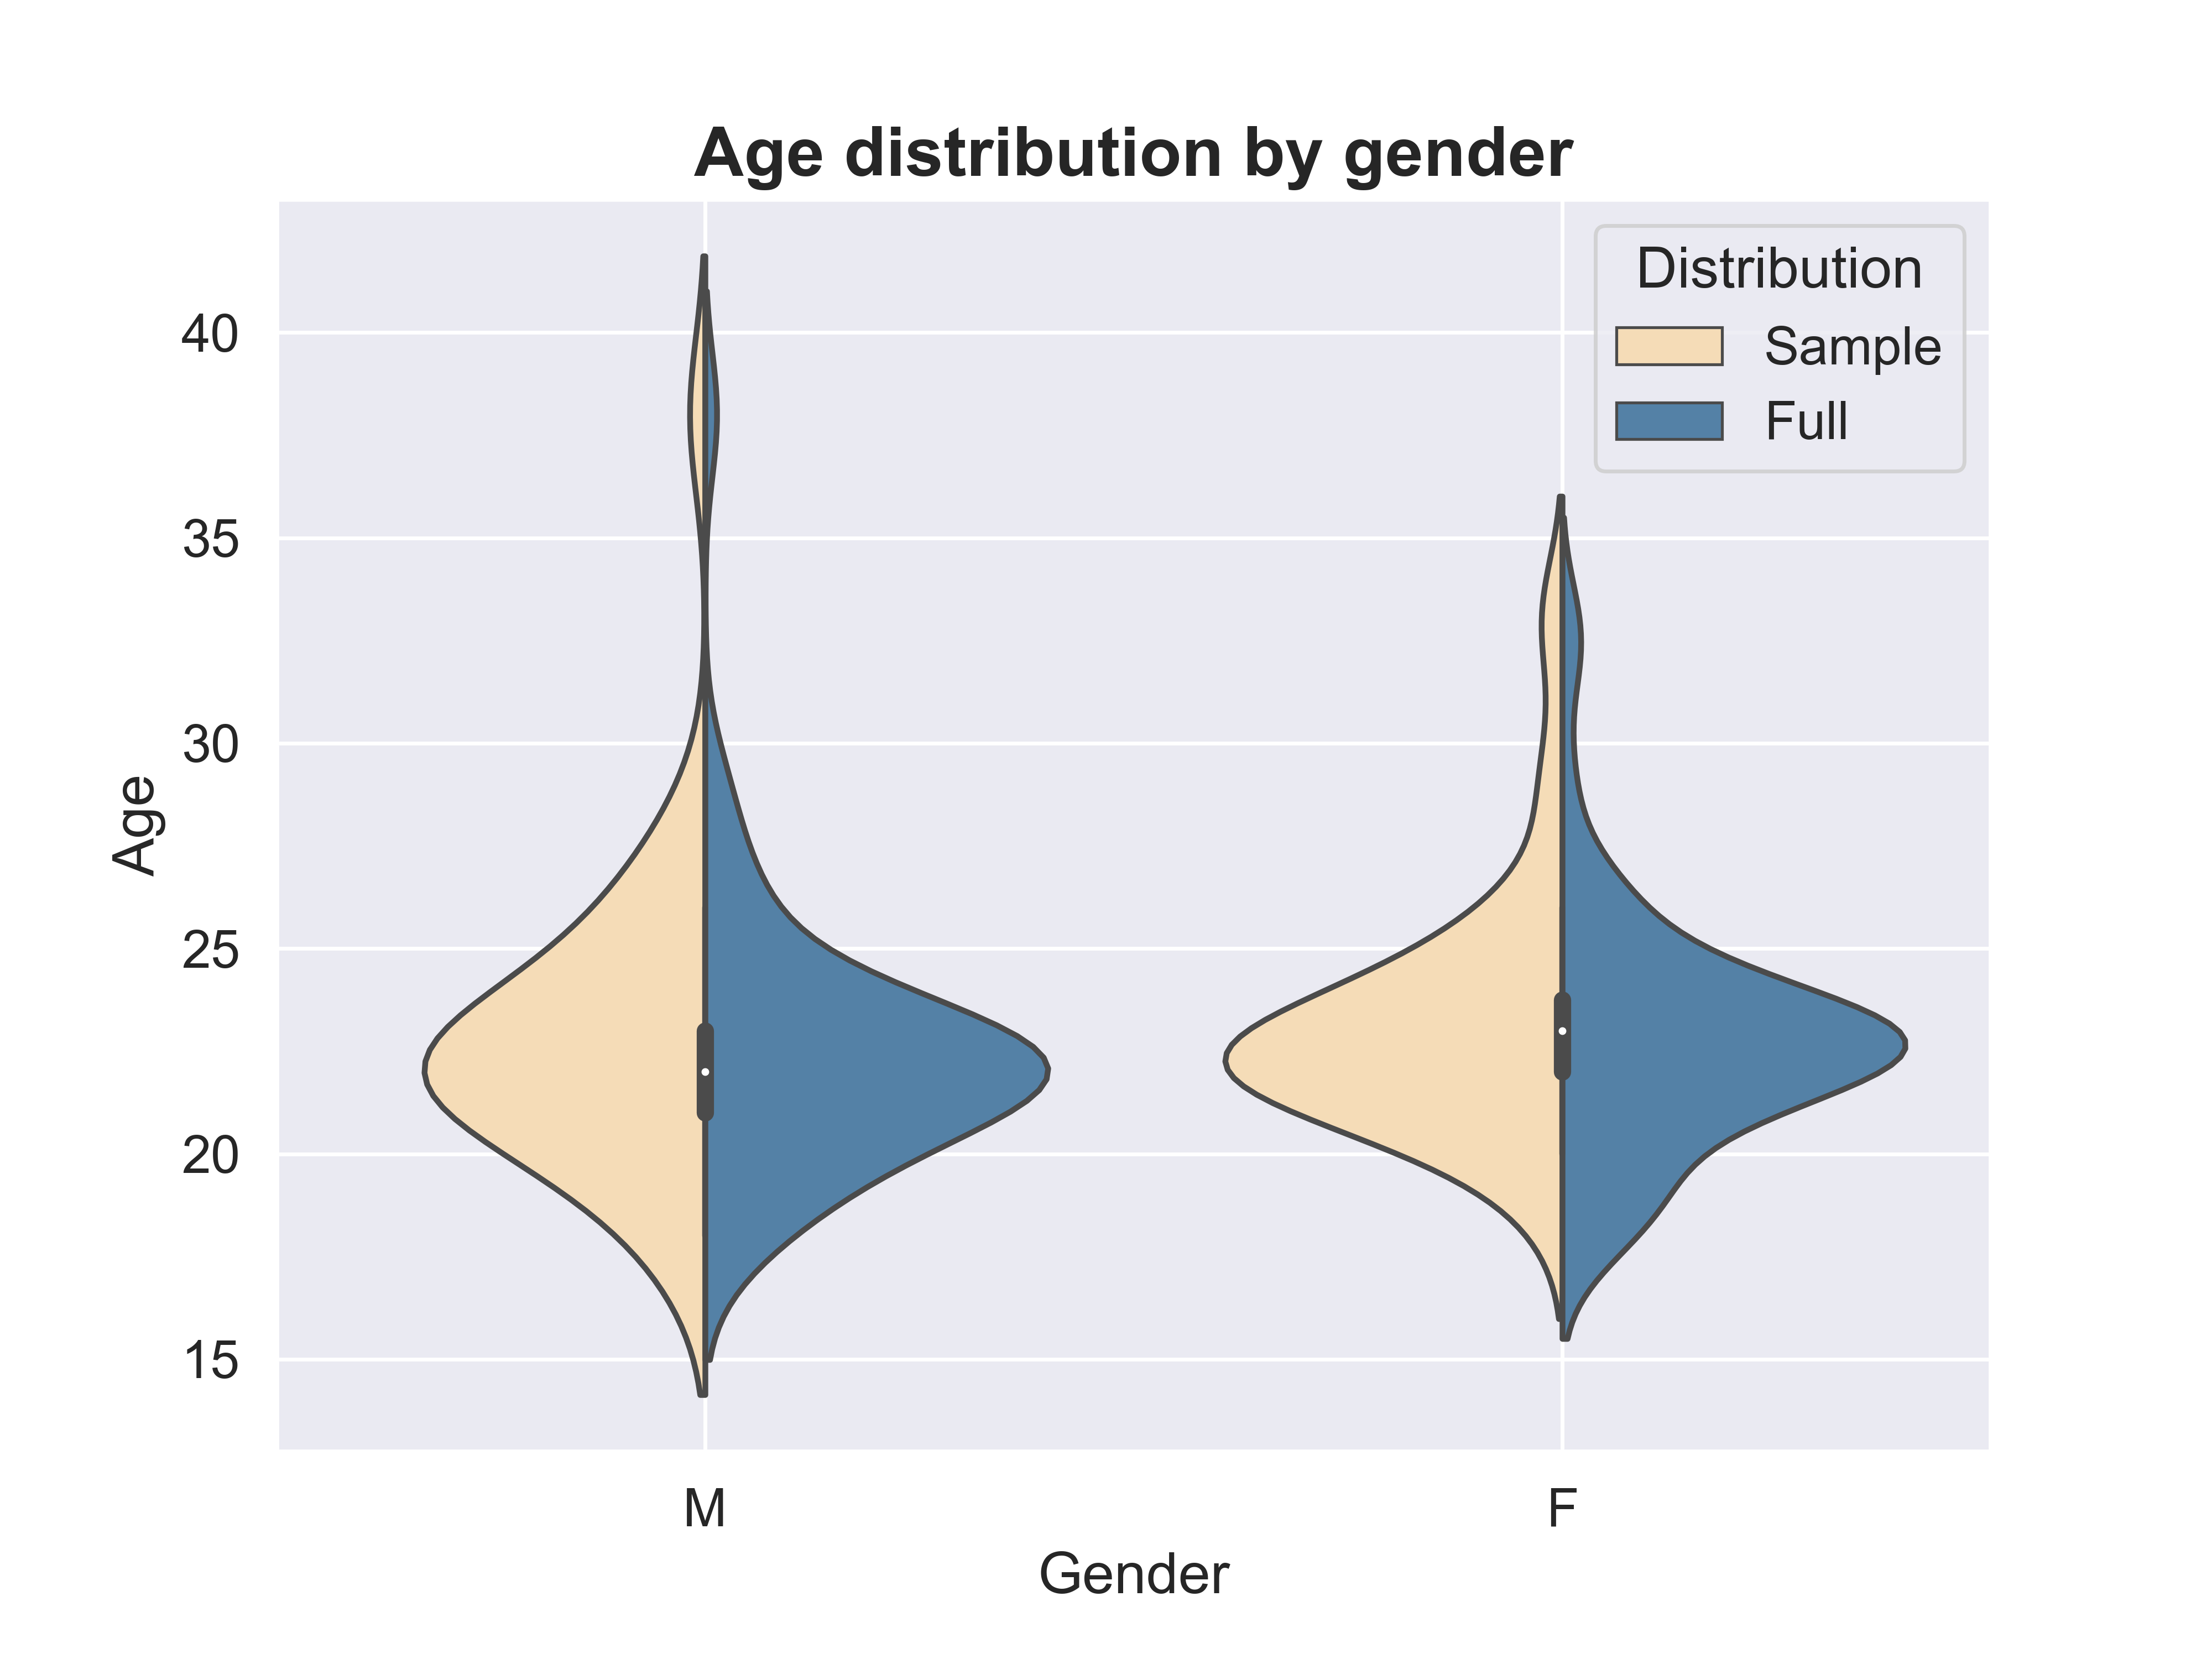
\includegraphics[scale=0.6]{img/age_distribution_by_gender.png}
		\caption{Violin plot showing the age distribution of speakers in \gls{vctk} dataset based on level of gender.}
		\label{fig:age_dataset}
	\end{center}
\end{figure}
\noindent As for the single-speaker task, we follow the previous works \cite{lim2018time} by indicating with "\gls{vctk}s" the subset of the whole dataset which only includes the first speaker. It is worth mentioning that this subset does not belong to the set of data used to train, validate or test the models for the multi-speaker task. The train-test split criterion is the same as the one used in both reference papers, i.e. a standard 85\% training - 15\% test split with no audio-clips overlap. \\
Furthermore, we keep the same data structure used in both \gls{tfnet} and \gls{tfilm} works: we extract from each recording a set of one-dimensional vectors of length 8192. In particular, each audio clip is divided into several subsequences by the use of a sliding window approach such that each subsequence (or \textit{patch}) shares 75\% of its content with the previous one. Therefore, recalling that the sampling rate of our data is 16 kHz, this corresponds to patches of approximately 500ms with the start of every patch 125 ms apart from the previous one. \\
The corresponding \gls{lr} patches are obtained by downsampling the original recordings. In particular, we use an order 8 Chebyshev type I low-pass filter with cut-off frequency at $R_{1_{lim}}$. Recalling that in our setup we have $R_1 = 4$ kHz, it follows that $R_{1_{lim}} = 2$ kHz. In other words, the low-pass filter allows to obtain the \gls{lr} signal by cutting off the frequency content of the \gls{hr} recording over the interval $\interval{R_{1_{lim}}}{R_{2_{lim}}} = \interval{4}{16}$ kHz. \\
Another preprocessing step consists in filtering silence sequences by discarding 256-length audio frames whose root-mean-square energy is below a fixed threshold of 0.05. Authors of \cite{lim2018time} find that this improves training convergences and stabilizes the gradient. In fact, conceptually it makes perfect sense not to train the model to increase the quality of silent audio data frames. This operation is performed only for the training set, and only in the multi-speaker task. \\
As mentioned in Chapter \ref{chap:methods}, we pre-process the \gls{lr} sequence via a cubic B-spline interpolation in order to obtain (\gls{lr},\gls{hr}) training pairs of the same length. This is one of the best approaches, among all non-adaptive techniques, that can be used to increase the temporal dimension of the input \cite{han2013comparison}. \\
Dataset statistics for both single and multi-speaker tasks are provided in Table \ref{tab:data_partition}. \\
\begin{table}[!htb]
	\begin{center}
		\begin{tabular}{@{}ccc@{}}
			\toprule
			\multicolumn{1}{c}{\textbf{Experiment}} &
			\multicolumn{1}{c}{\textbf{Portion}} &
			\multicolumn{1}{c}{\textbf{n. of patches}} \\ \midrule
			Single-Speaker & Train & 6,656\\
			& Test & 768\\
			Multi-Speaker & Train & 129,920 \\
			& Validation & 40,448 \\
			& Test & 78,592 \\ \bottomrule
		\end{tabular}
		\caption{Data partition details for both \textit{Single-Speaker} and \textit{Multi-Speaker} tasks.}
		\label{tab:data_partition}
	\end{center}
\end{table}

\subsection{Training Details} \label{training_details}
This paragraph focuses on the training of the three models and the choice of their hyper-parameters. \\
Following the previous works (\cite{lim2018time}, \cite{birnbaum2019temporal}), we train all models using the Adam optimizer \cite{kingma2014adam} with learning parameters $\beta_1 = 0.9, \beta_2 = 0.999, \epsilon = 10^{-7}$ and a batch size of 128. \\
As for the learning rate, we use different approaches; Lim, Yeh et al.\cite{lim2018time} propose a starting learning rate of $3\times 10^{-5}$ with a polynomial decay scheduling with rate of 0.5. We use this setup for both \gls{tfnet} and the proposed model. As for \gls{tfilm} Net, we use the constant value of $10^{-5}$ which is proposed by its authors. Consequently, this causes a different time for training: \gls{tfilm} net convergence speed is slower because of its lower learning rate. In fact, the total number of epochs to finish the training is higher in \gls{tfilm} net, as we can see in Figure \ref{fig:tfilmnet_training_curves}. \\
In this regard, it is important to highlight how the criterion for determining the total number of steps is chosen: for this decision we use a validation set along with the early stopping criteria. Intuitively, it is possible to consider this setting as a hyperparameter selection method, where the total number of steps is the hyperparameter to be optimized. The interruption criteria is as follows: the model training is interrupted if neither the loss nor the \gls{snr} (which is described in paragraph \ref{eval_methods}) improve within 25,000 consecutive steps (which correspond to 24 epochs). Training curves for the Multi-Speaker task are shown in figures \ref{fig:tfnet_training_curves}, \ref{fig:tfilmnet_training_curves}, \ref{fig:proposed_training_curves}. \\

\begin{figure}[!htb]
	\begin{subfigure}{.5\textwidth}
		\centering
		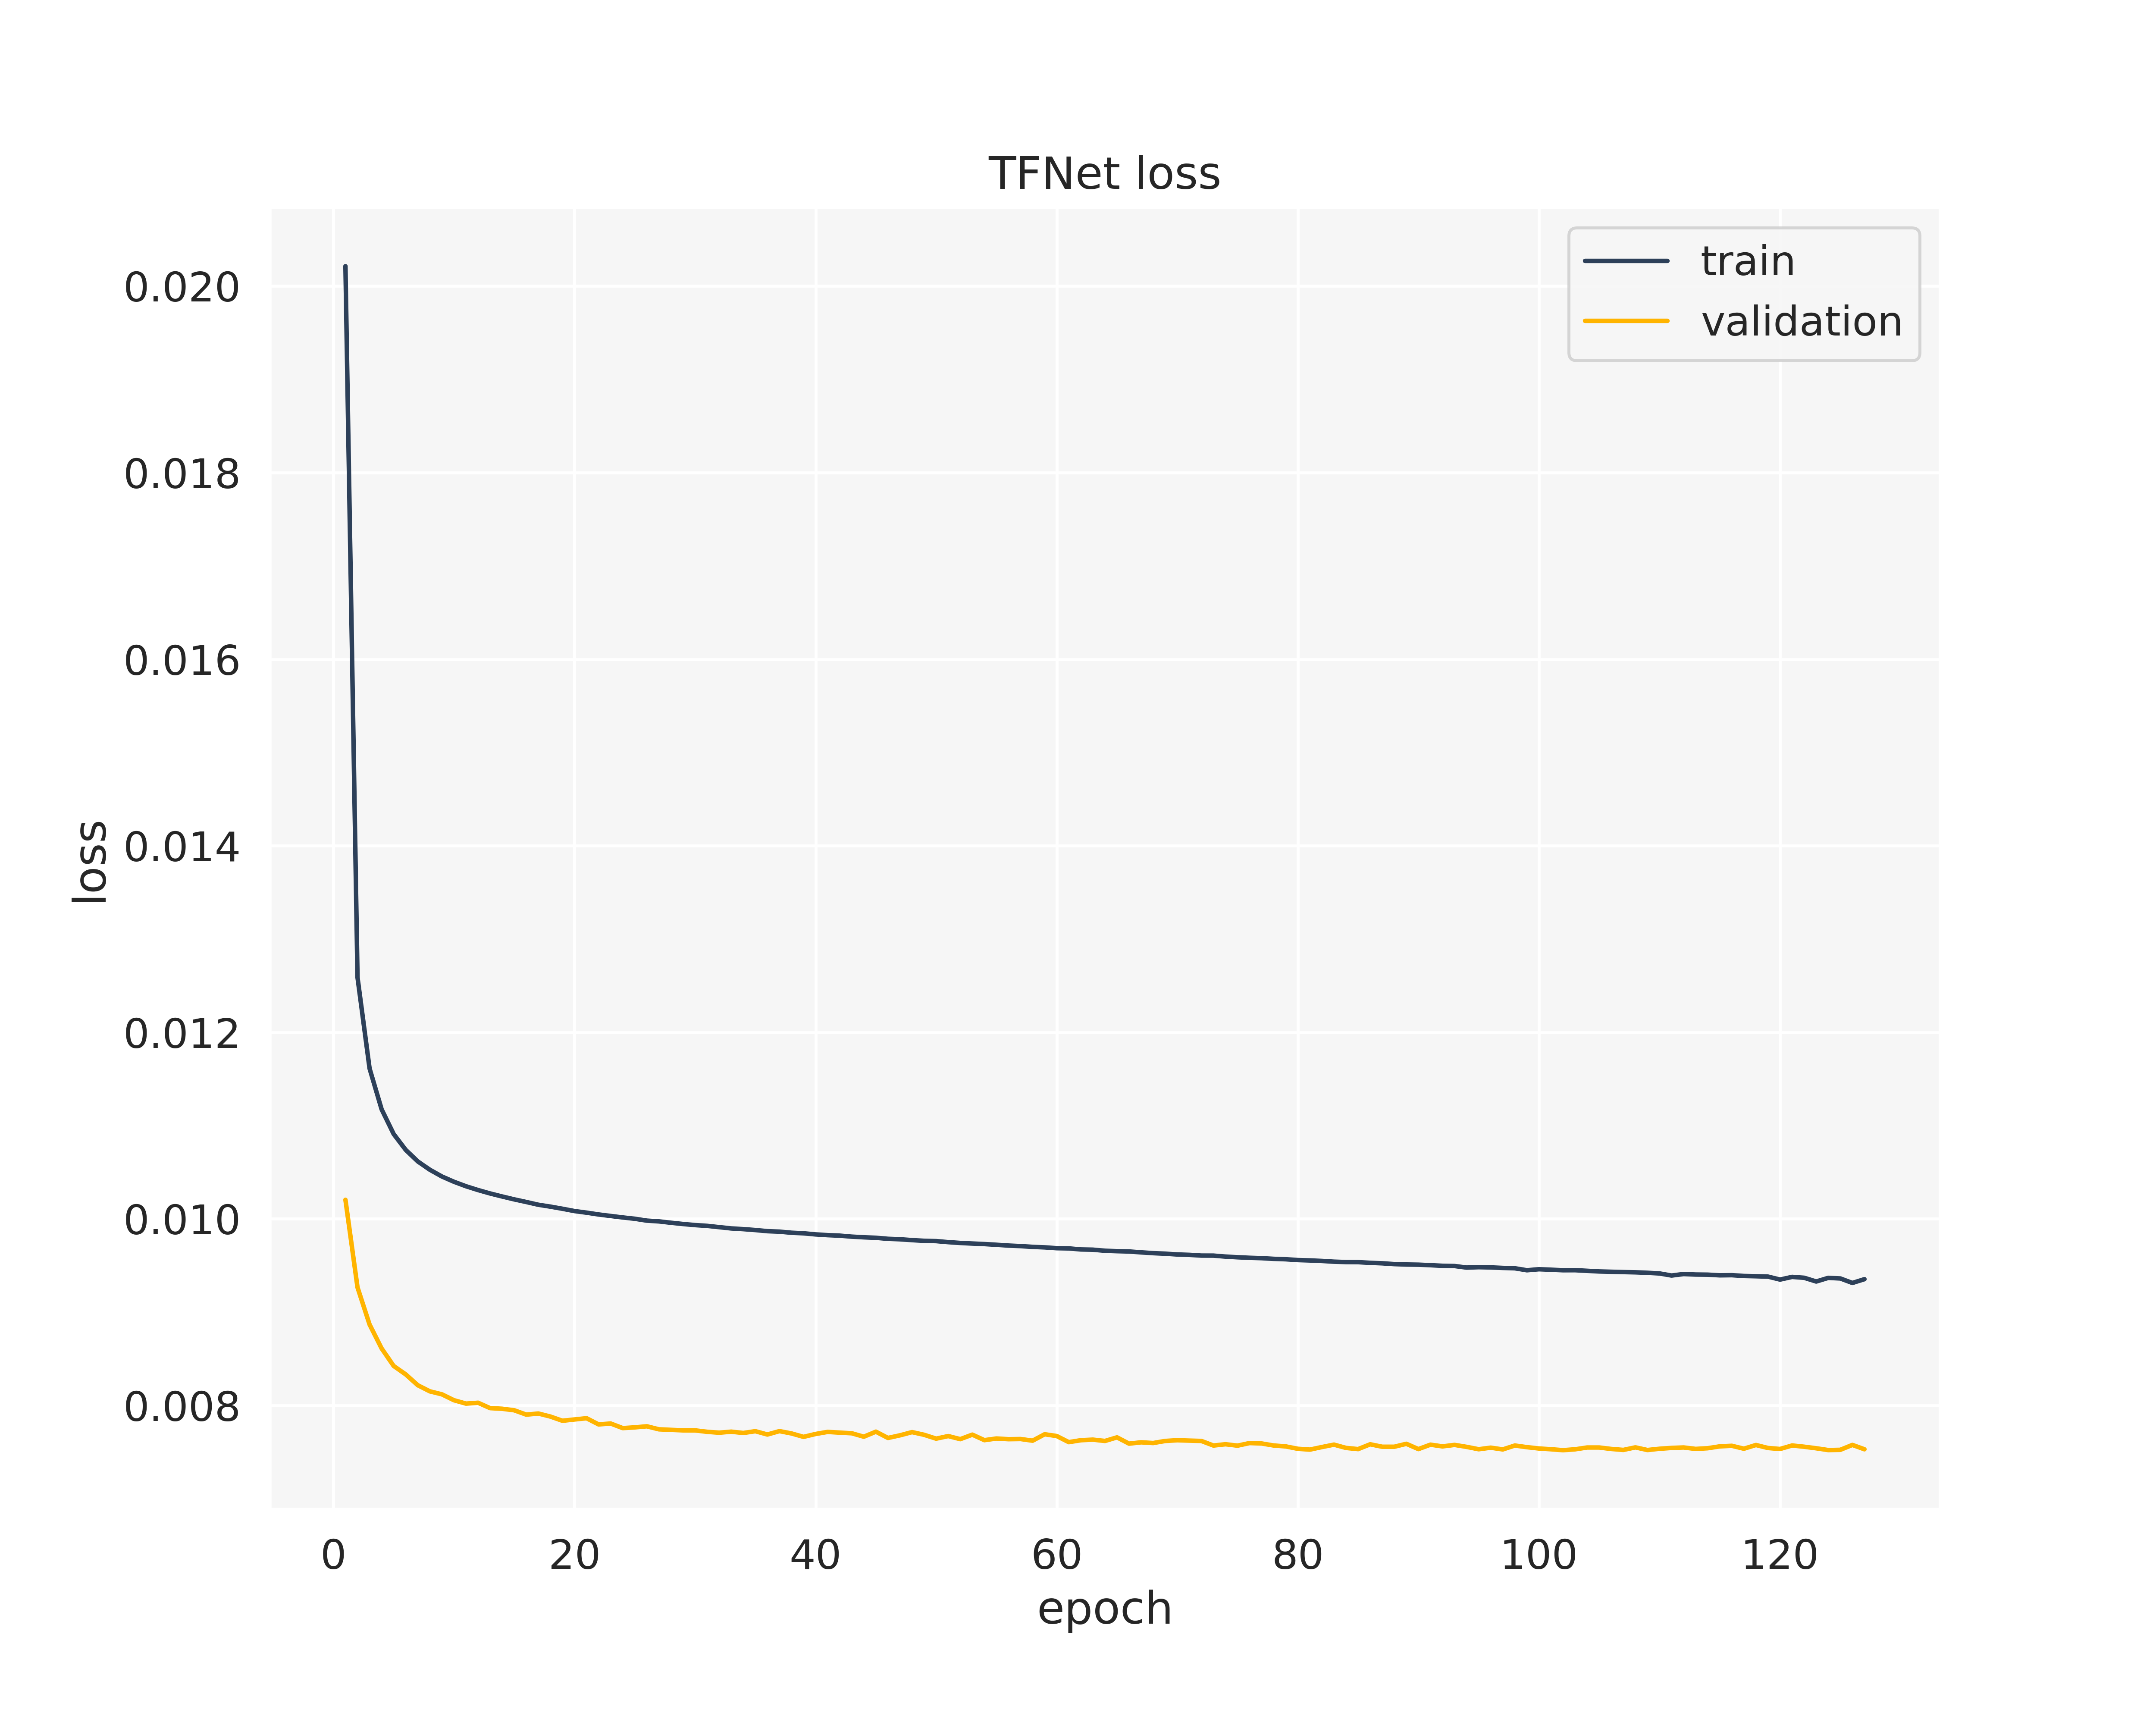
\includegraphics[width=1.05\linewidth]{img/tfnet_loss.png}
		\label{fig:tfnet_loss}
	\end{subfigure}%
	\begin{subfigure}{.5\textwidth}
		\centering
		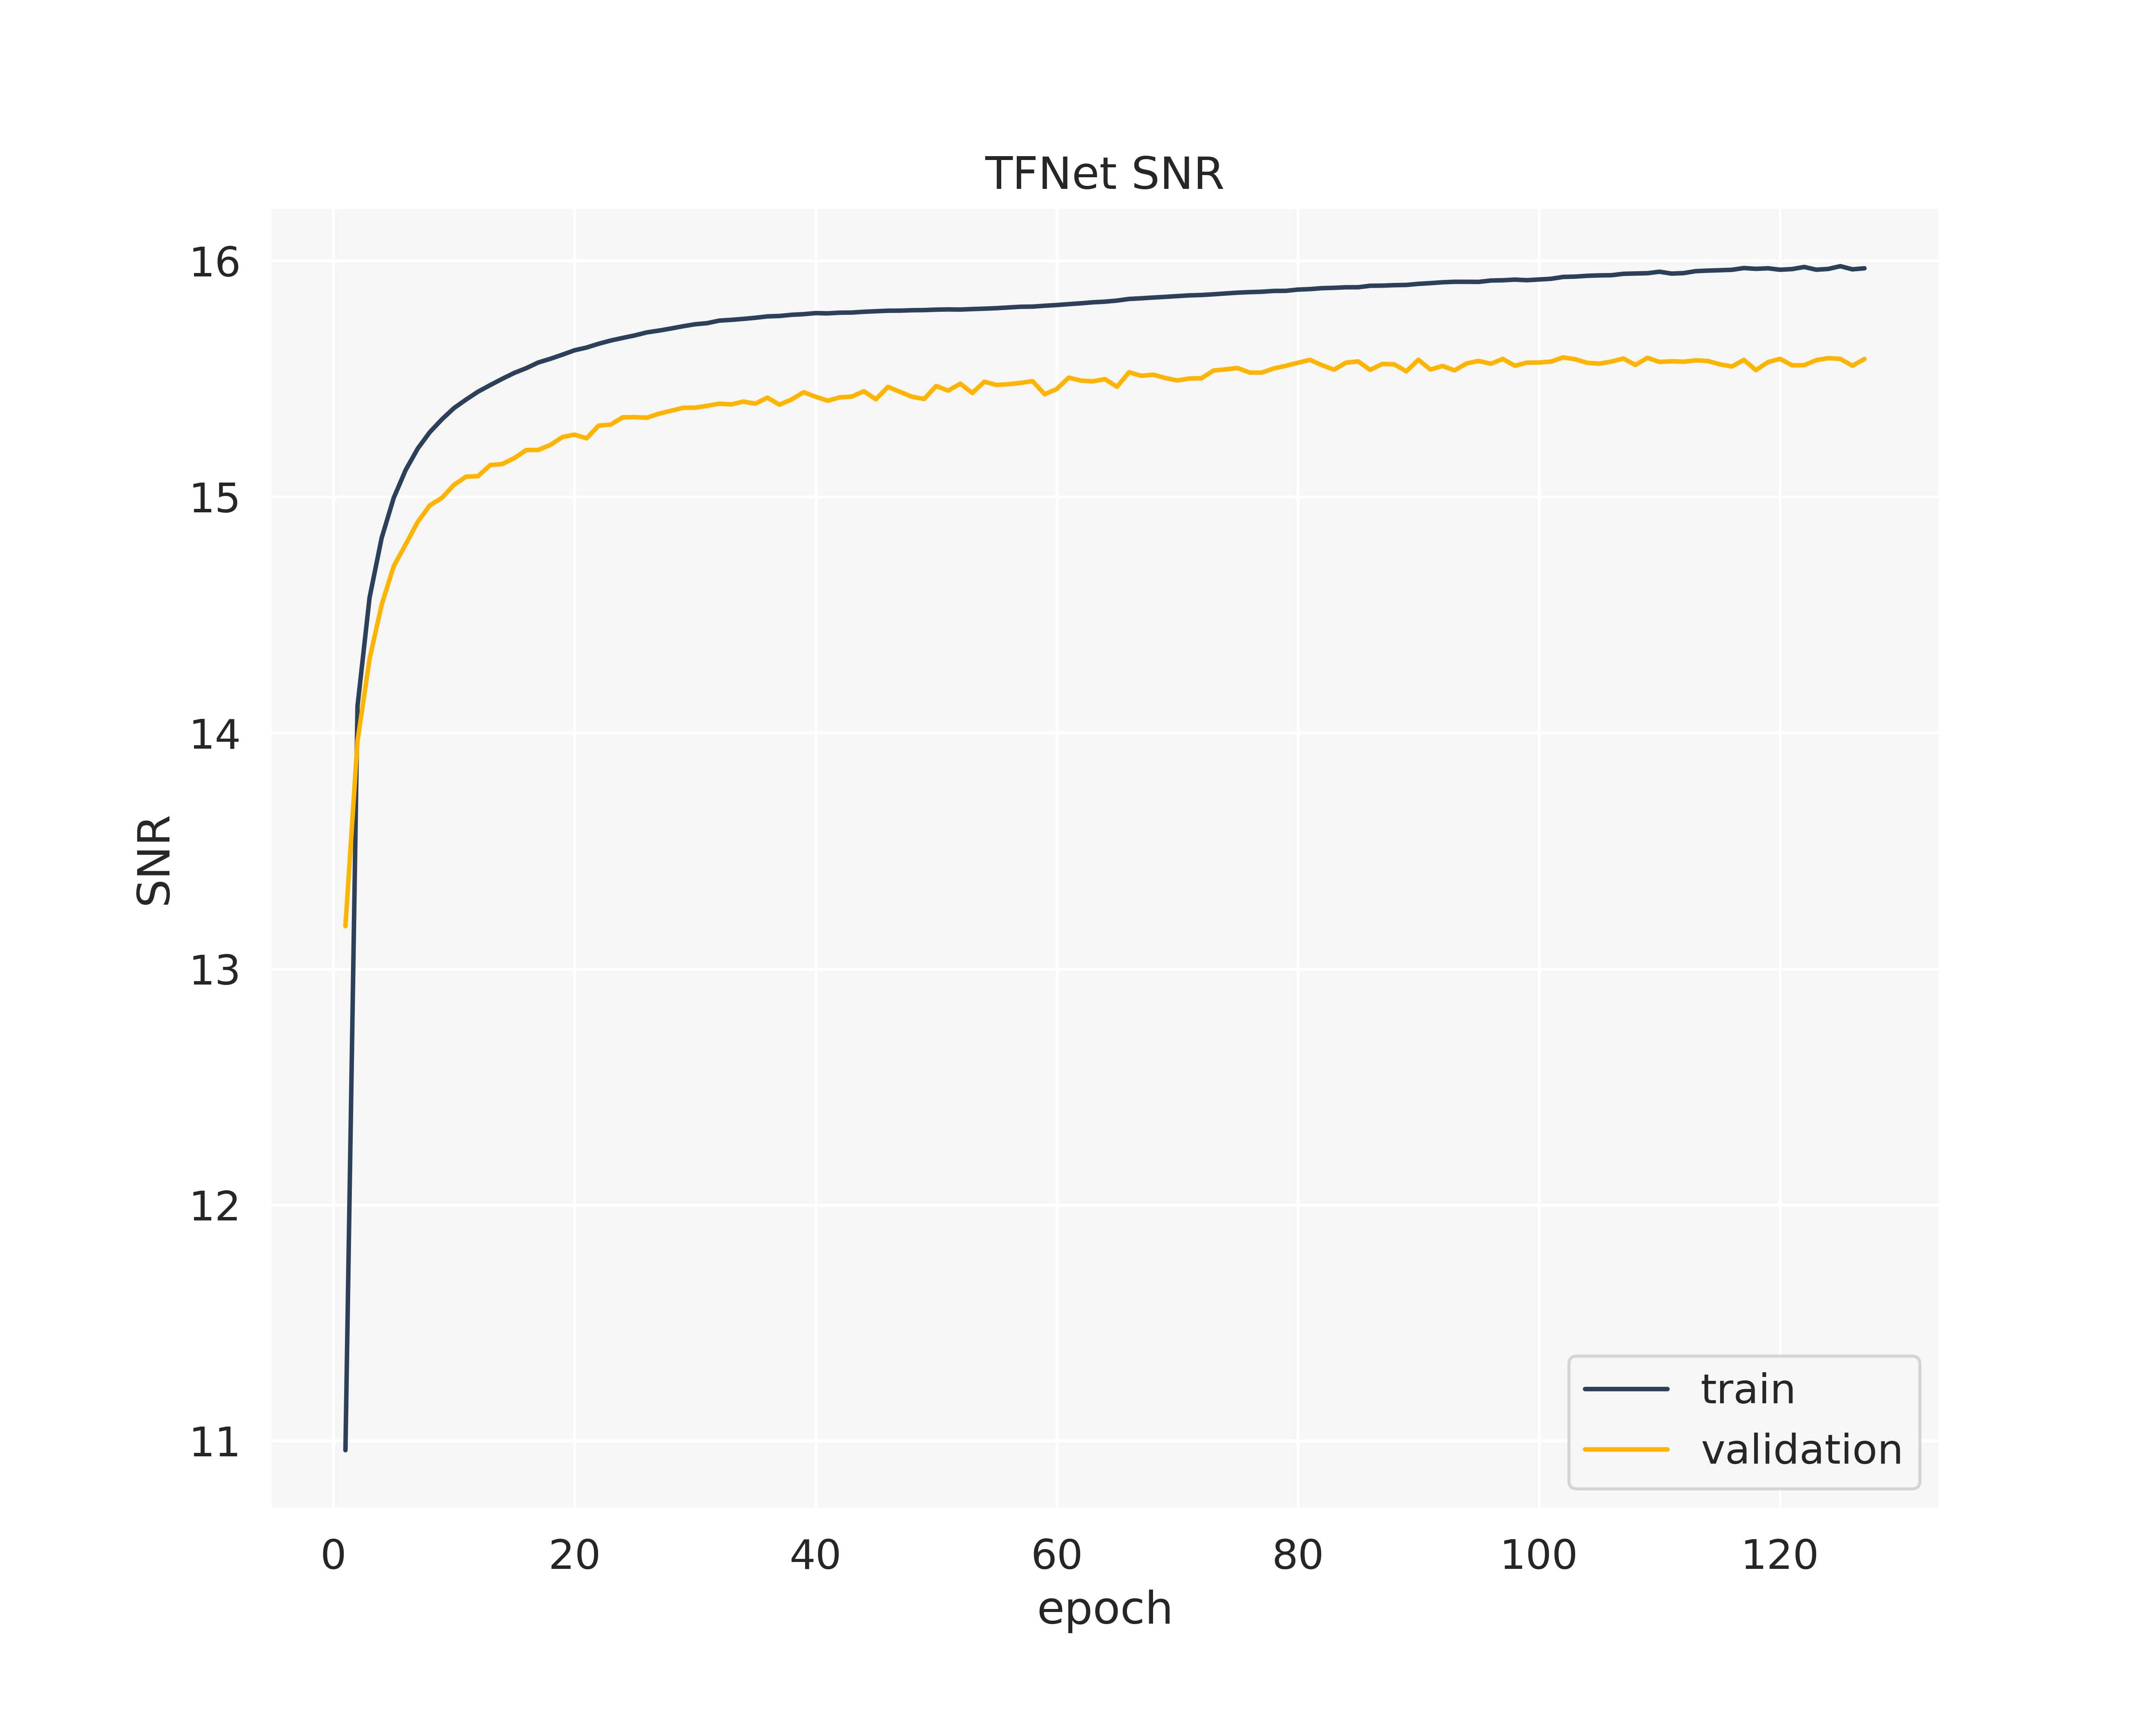
\includegraphics[width=1.05\linewidth]{img/tfnet_snr.png}
		\label{fig:tfnet_snr}
	\end{subfigure}%
	\caption{\gls{tfnet} training curves on both training and validation sets. The model is trained for 127 epochs.}
	\label{fig:tfnet_training_curves}
\end{figure}

\begin{figure}[!htb]
	\begin{subfigure}{.5\textwidth}
		\centering
		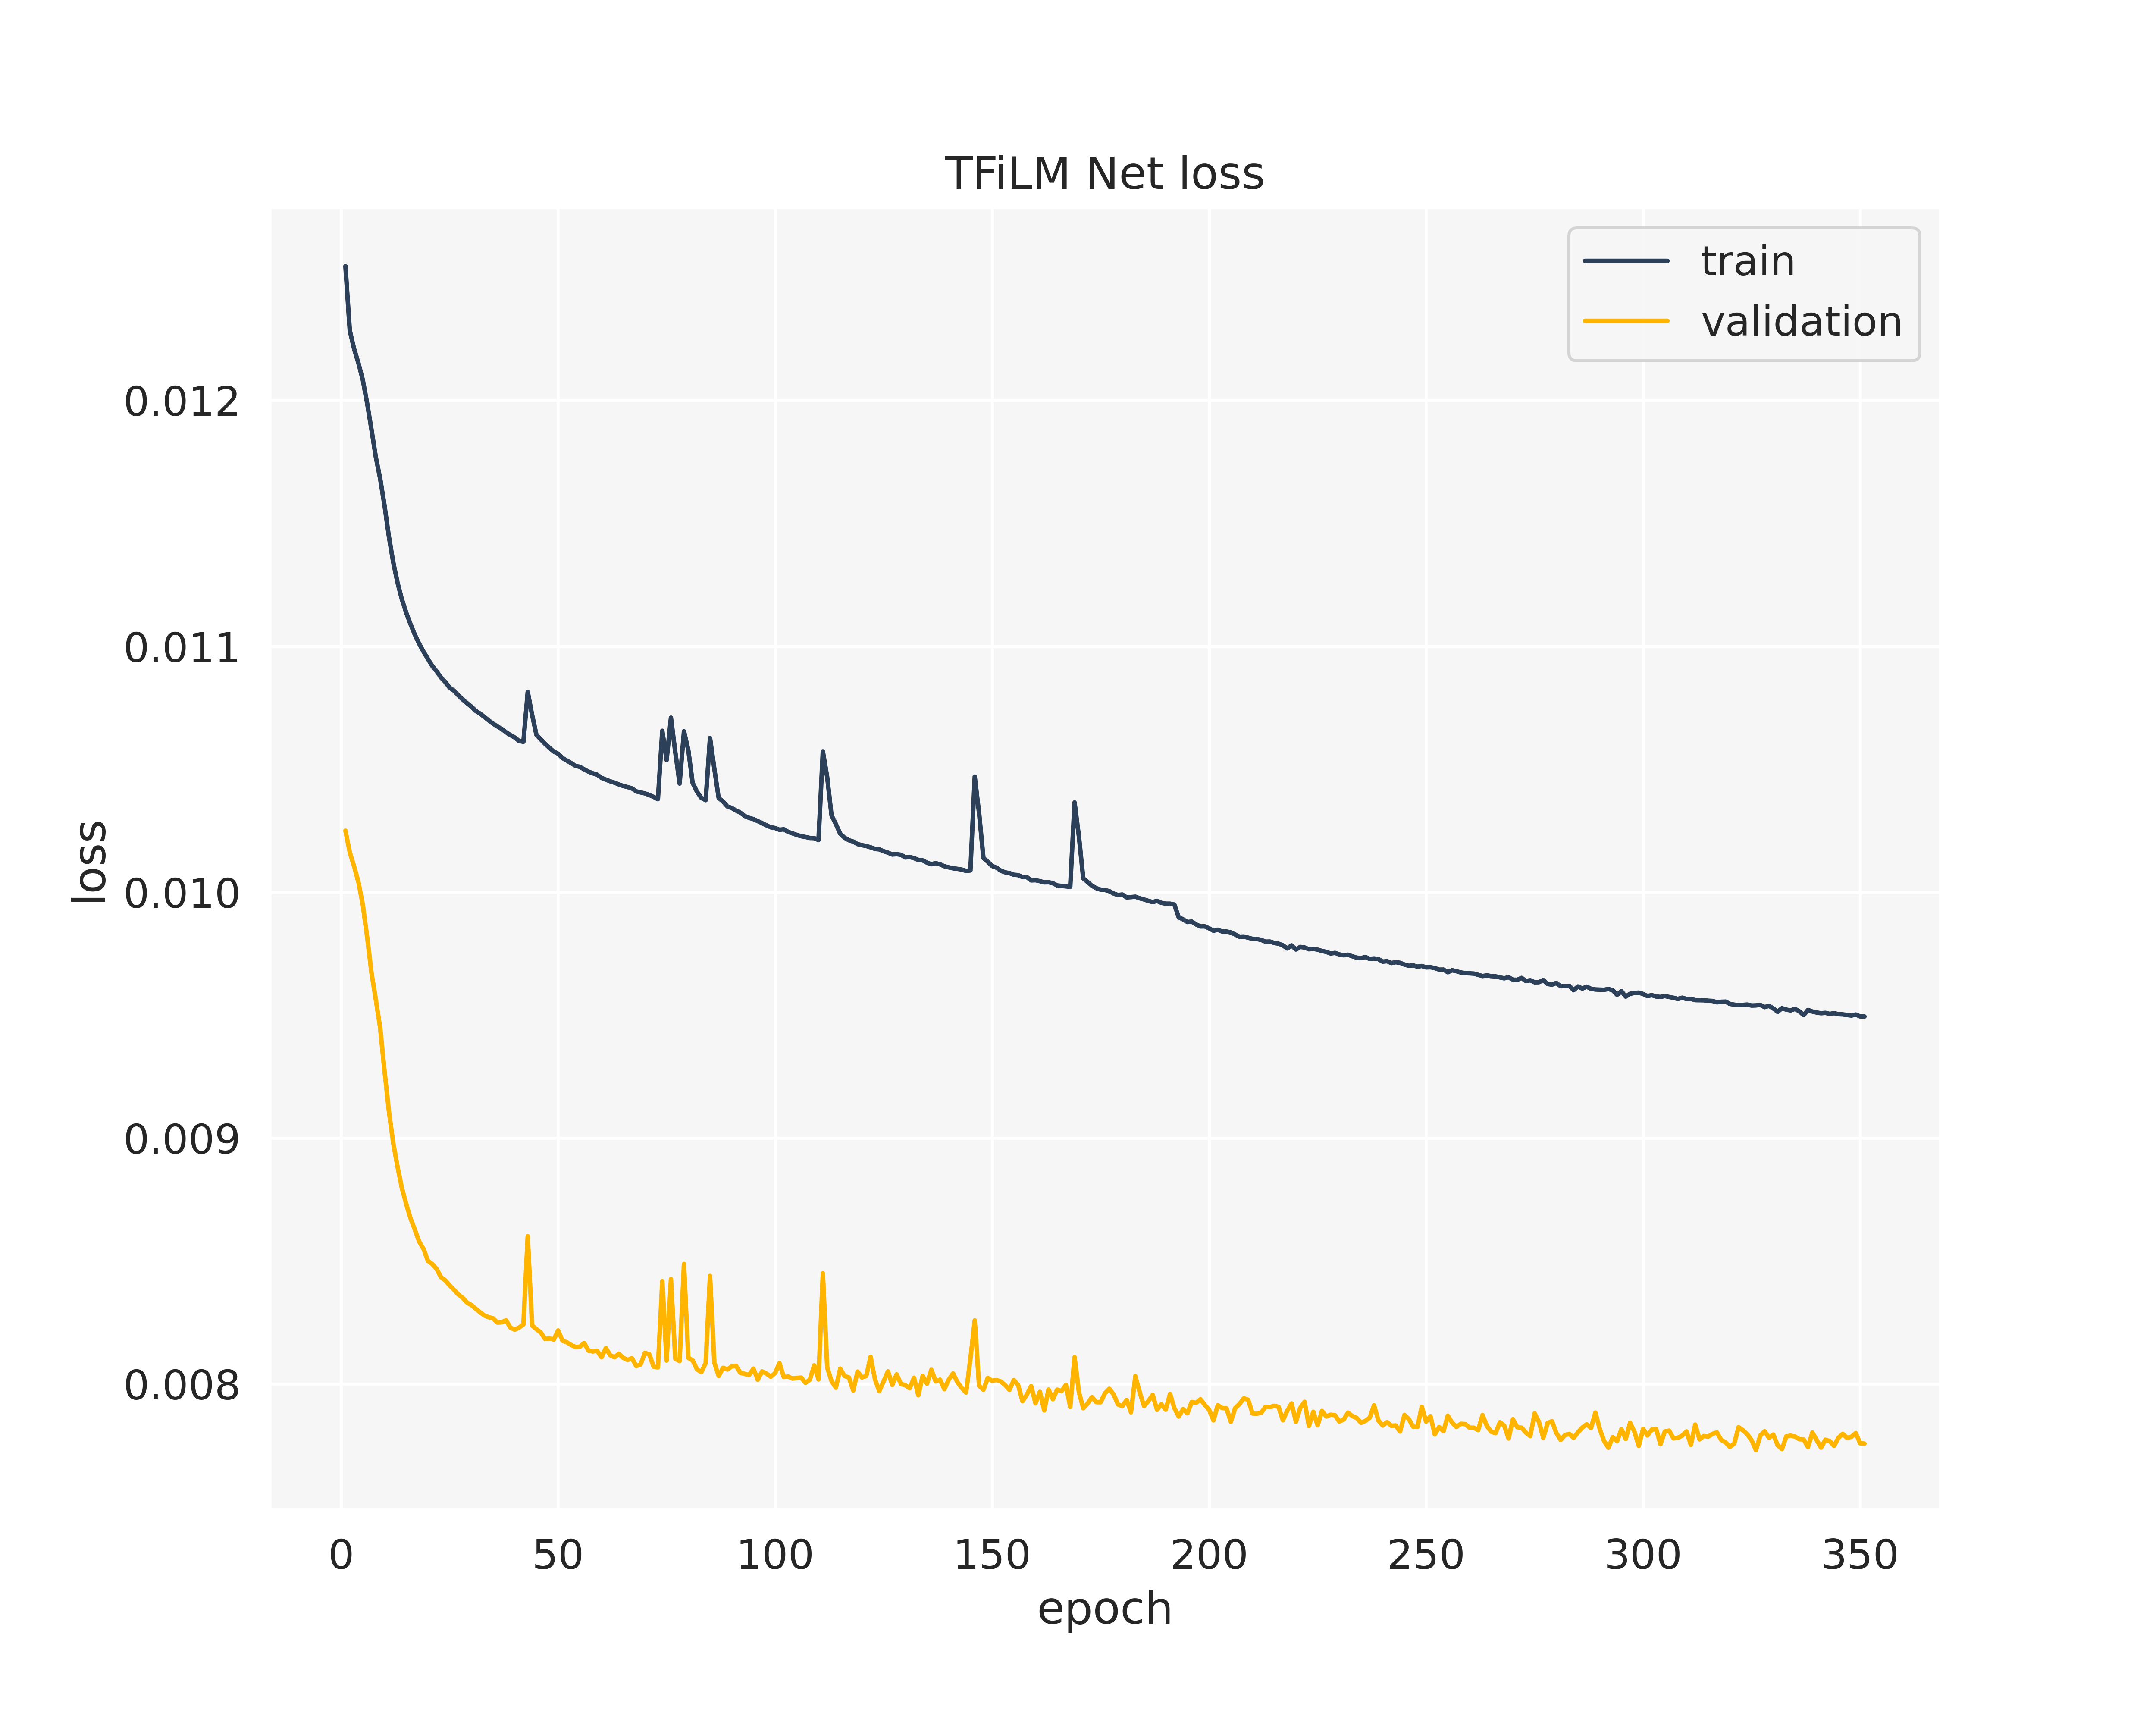
\includegraphics[width=1.05\linewidth]{img/tfilmnet_loss.png}
		\label{fig:tfilmnet_loss}
	\end{subfigure}%
	\begin{subfigure}{.5\textwidth}
		\centering
		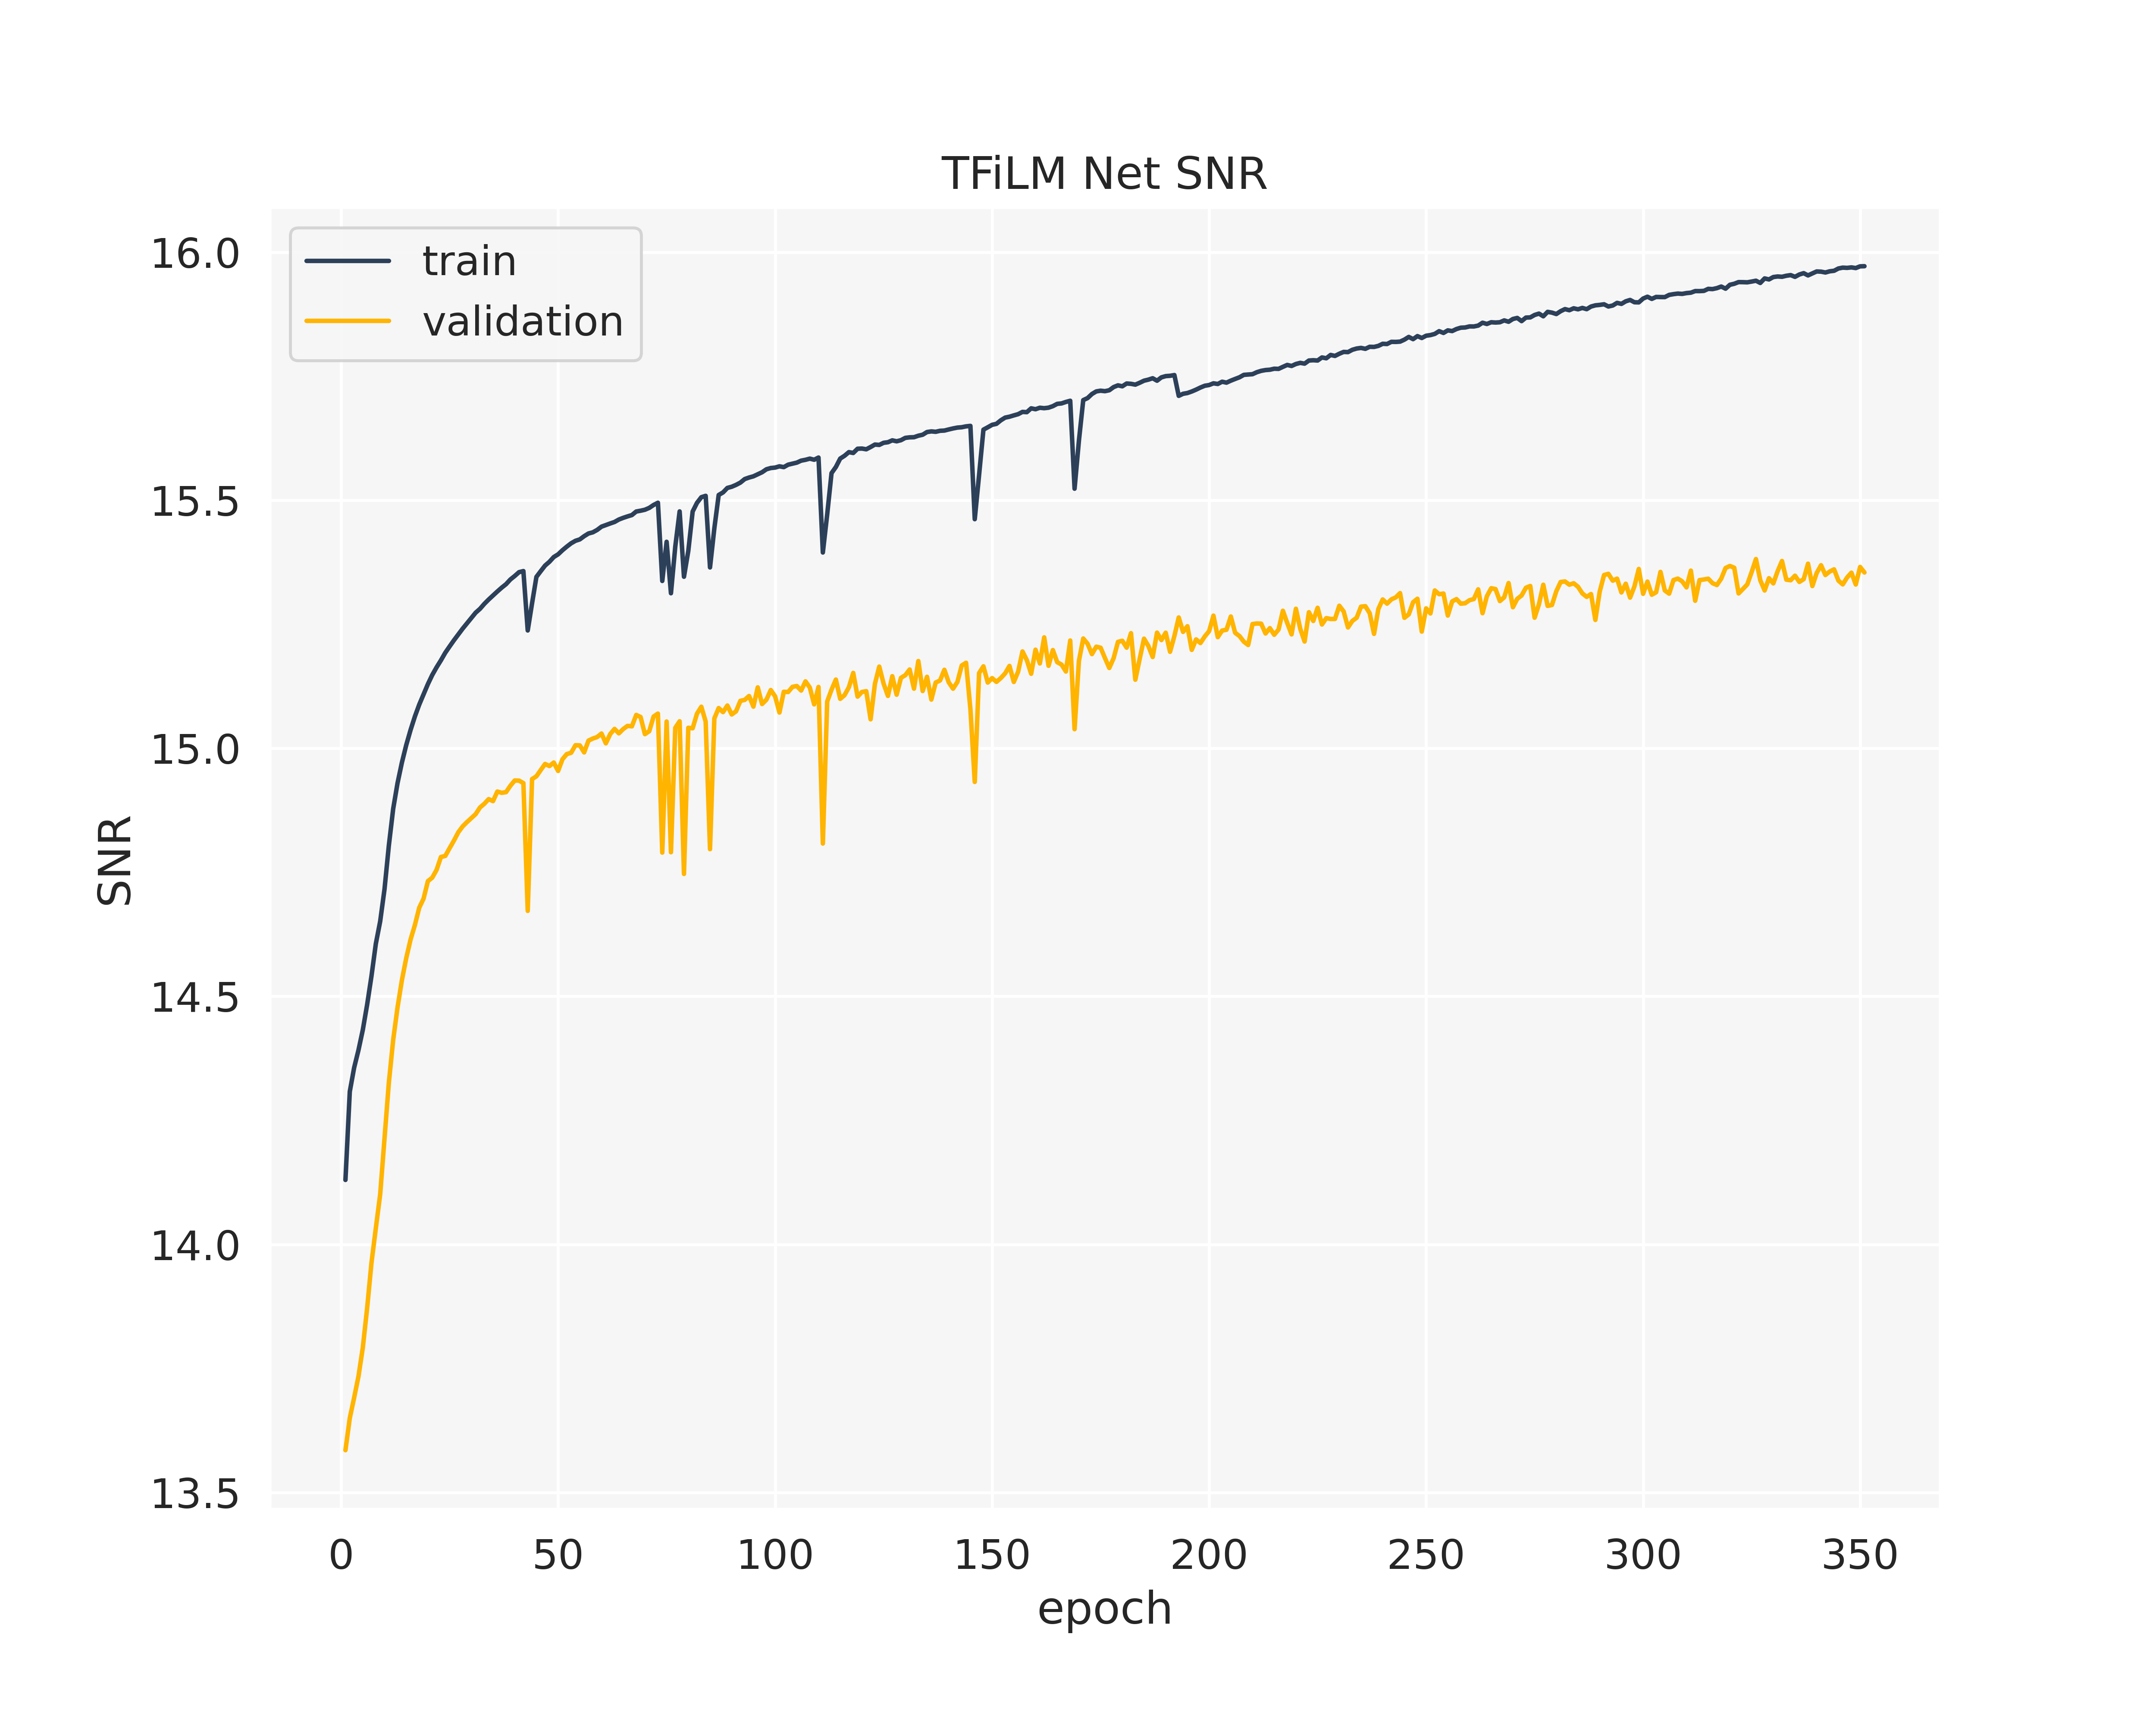
\includegraphics[width=1.05\linewidth]{img/tfilmnet_snr.png}
		\label{fig:tfilmnet_snr}
	\end{subfigure}%
	\caption{\gls{tfilm} Net training curves on both training and validation sets. The model is trained for 351 epochs.}
	\label{fig:tfilmnet_training_curves}
\end{figure}

\begin{figure}[!htb]
	\begin{subfigure}{.5\textwidth}
		\centering
		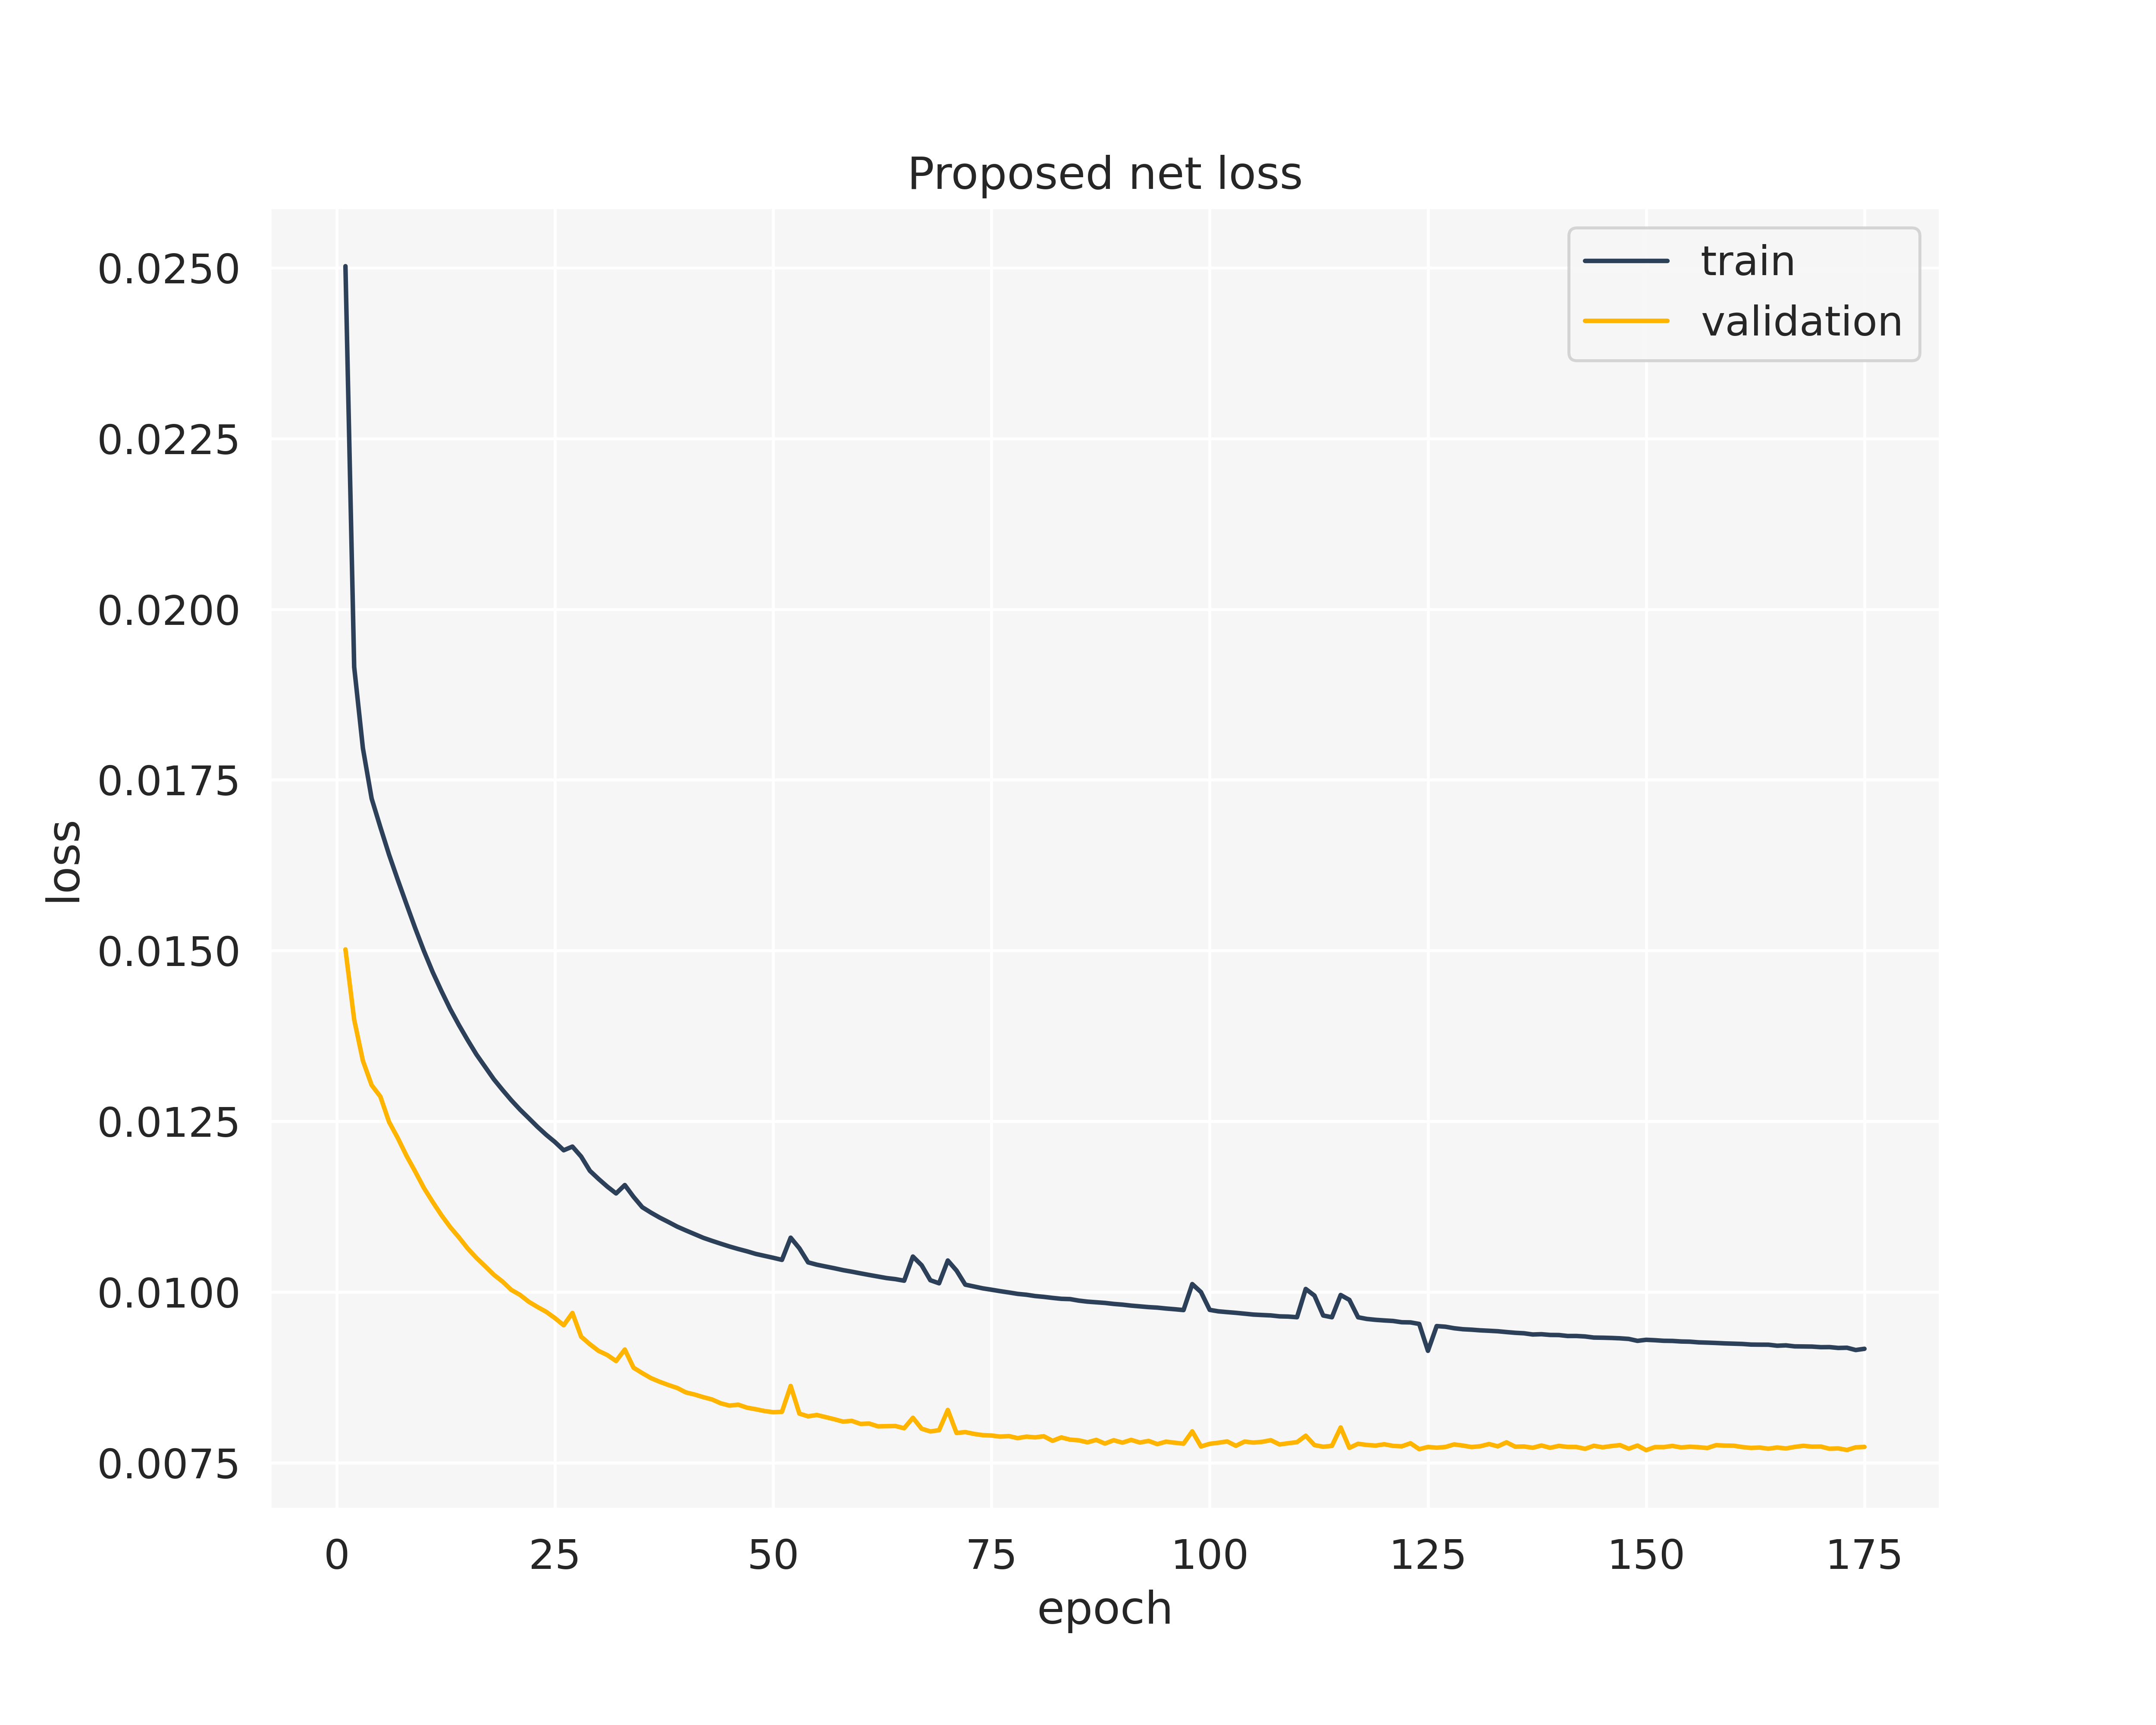
\includegraphics[width=1.05\linewidth]{img/gionet_loss.png}
		\label{fig:gionet_loss}
	\end{subfigure}%
	\begin{subfigure}{.5\textwidth}
		\centering
		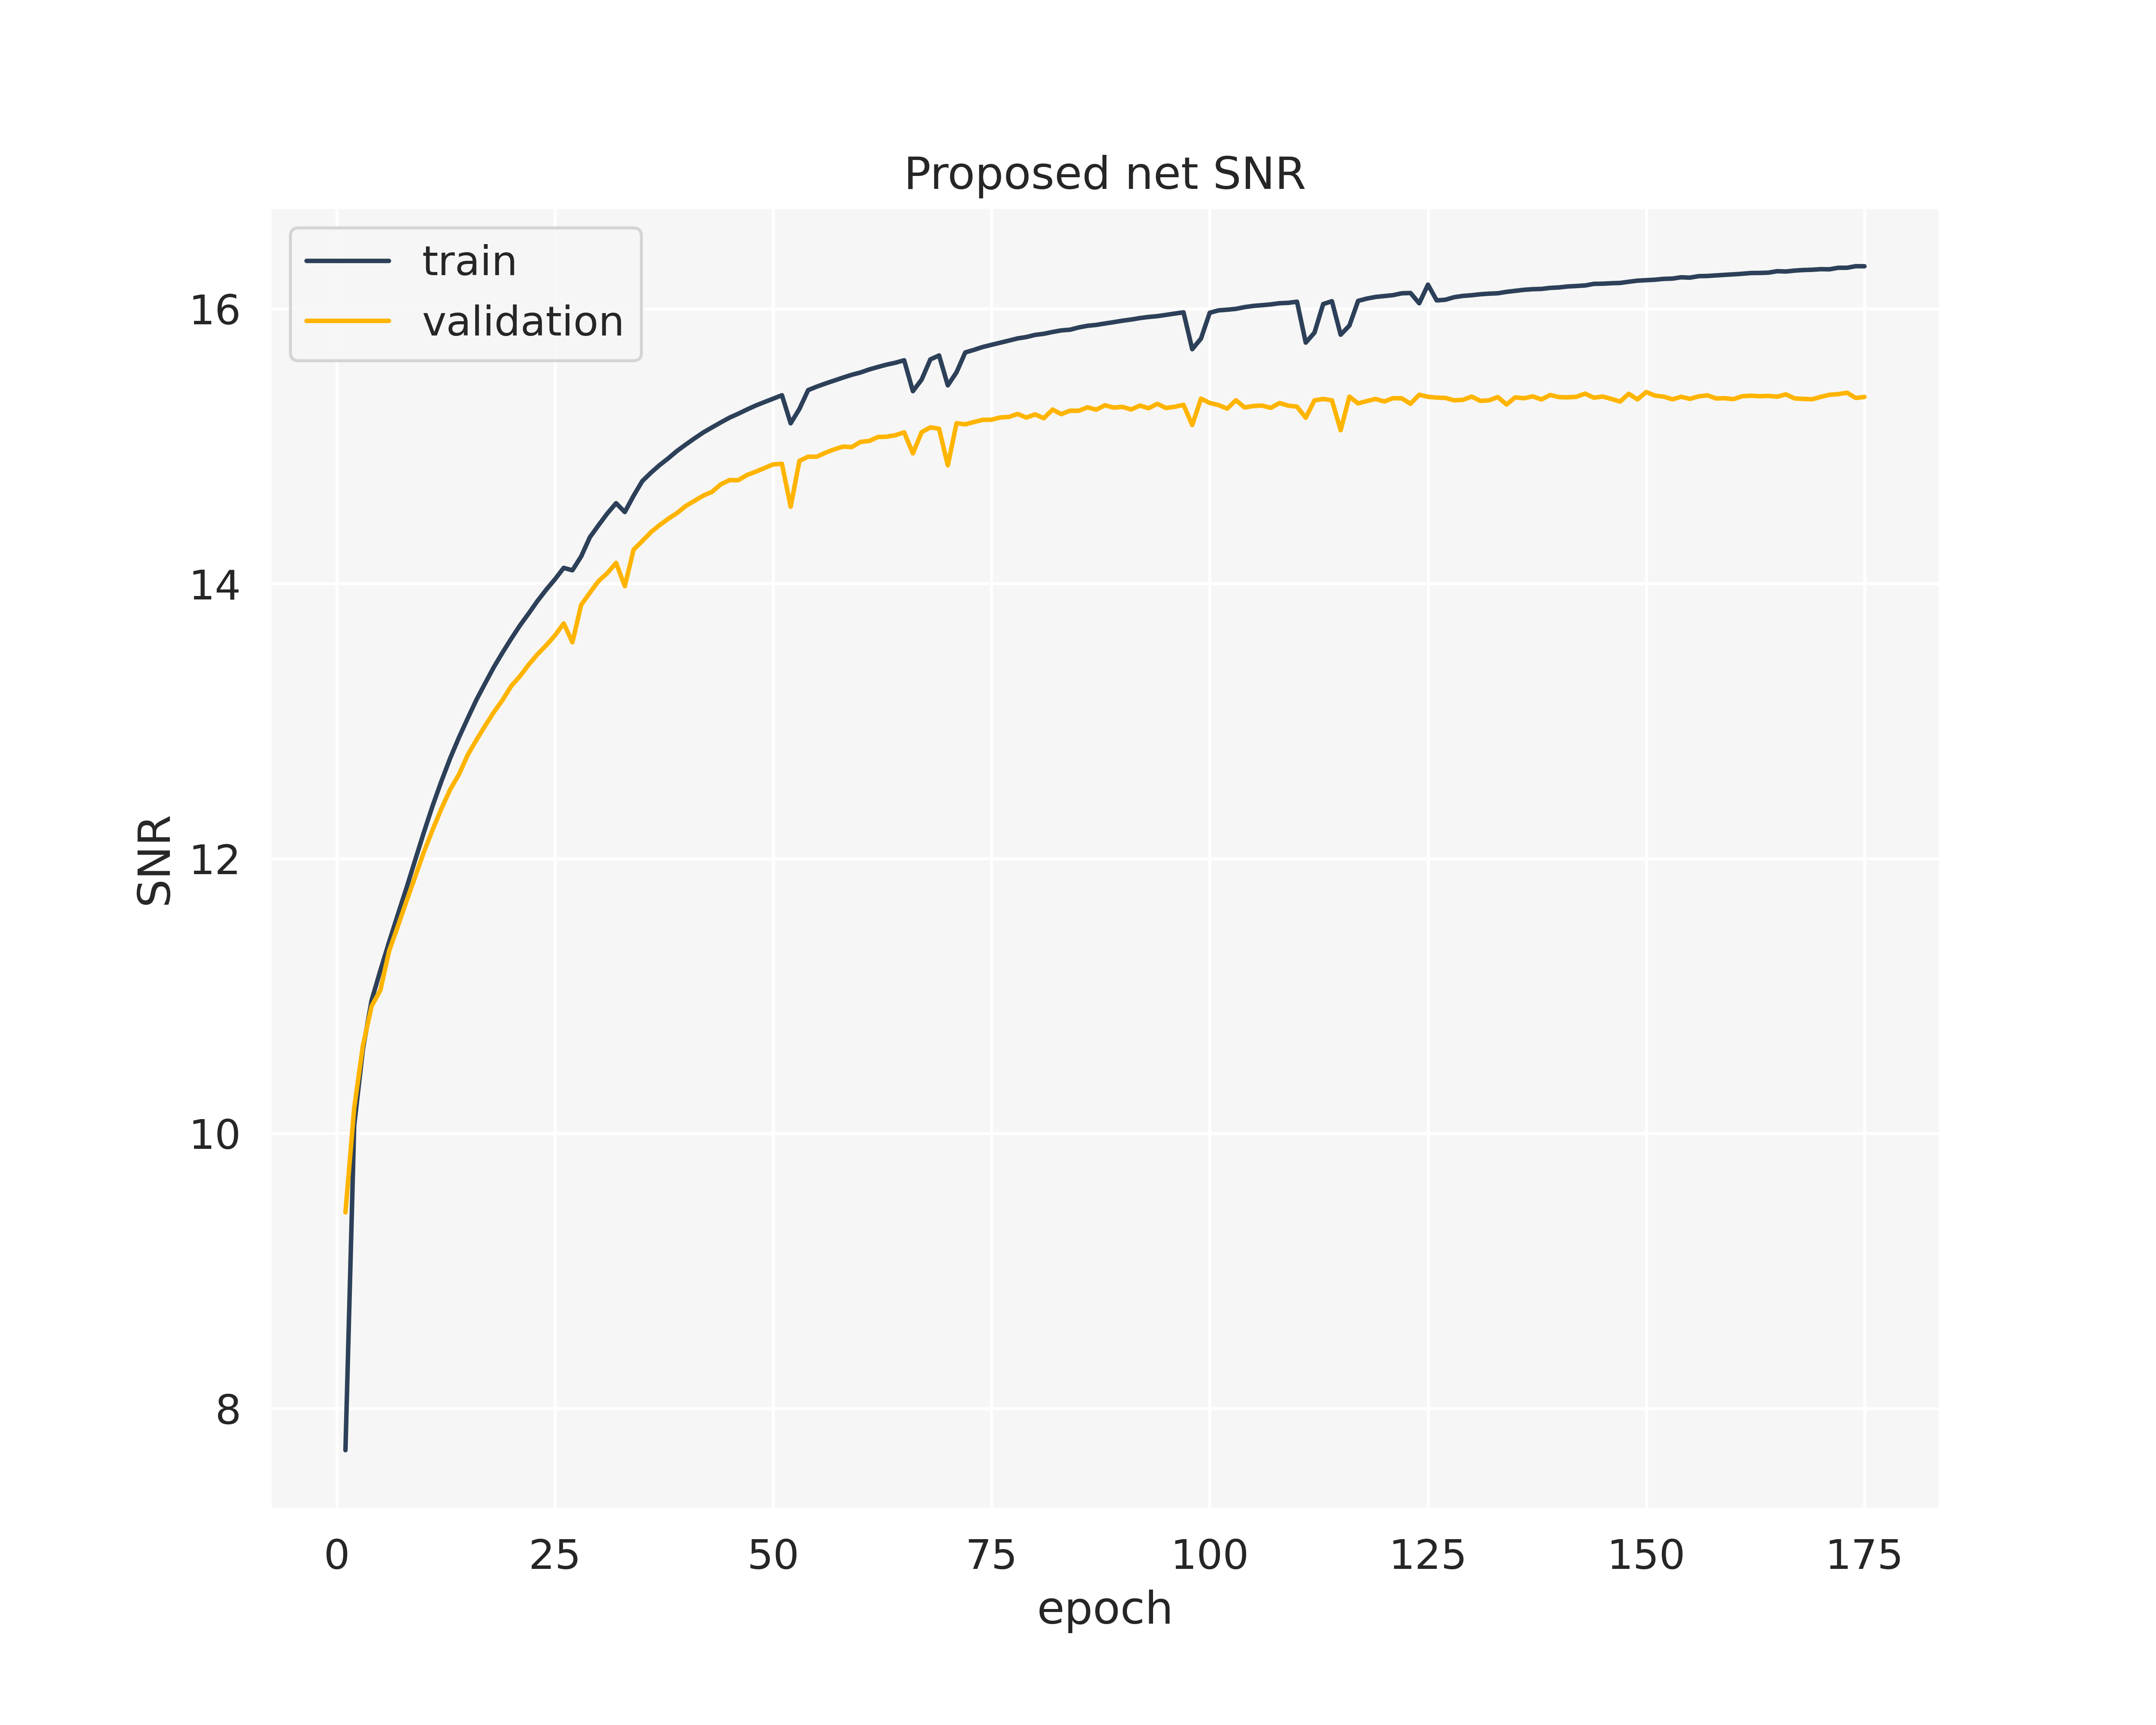
\includegraphics[width=1.05\linewidth]{img/gionet_snr.png}
		\label{fig:gionet_snr}
	\end{subfigure}%
	\caption{Proposed net training curves on both training and validation sets. The model is trained for 175 epochs.}
	\label{fig:proposed_training_curves}
\end{figure}

\noindent We can see that although the loss values in the validation set are better than in the training set, the \gls{snr} value is generally lower. This may be due to the different data distribution in the two sets; in fact, we remind that in the validation set there are more silence audio frames, which instead are filtered from training data.\\
Another relevant aspect is the following: initially, each model is trained on the Multi-Speaker task. Subsequently, Single-Speaker models are obtained through a \textit{fine tuning} operation of the previously trained models. Fine tuning consists in training a pre-trained model on a smaller dataset. More specifically, it is the practice of using pre-trained weights from a model trained on a large dataset (in our case, the \gls{vctk} corpus) as a starting point for a different dataset (\gls{vctk}s). By doing so, we exploit a greater power of generalization (the one of Multi-Speaker models) instead of starting from scratch. \\
It is worth stressing that the optimizer, the number of training steps, the learning rate, and the other hyperparameters are kept the same for both Single-Speaker and Multi-Speaker regimes. Consequently, this results in a larger number of epochs for the Single-Speaker task since \gls{vctk}s is significantly smaller than \gls{vctk}. \\
Finally, we mention that in the Multi-Speaker we select as the final model configuration the one which corresponds to the last validation set improvement on either the loss or the \gls{snr} values. On the other hand, in the Single-Speaker task, since there is no validation set, we simply take the model weights at the last epoch.

\subsection{Evaluation Methods} \label{eval_methods}
In this section the metrics used to evaluate the models introduced in Chapter \ref{chap:methods} are presented. We use two standard metrics used in the audio \gls{sr} literature such as \gls{snr} and \gls{lsd} \cite{gray1976distance}. While the former takes into account a weighted difference between the model signal reconstruction and the ground-truth data in the time domain, the latter measures the reconstruction quality in the frequency domain. \\
More specifically, \gls{snr} is the ratio, usually expressed on a logarithmic scale in decibels, between the signal power level and the noise power level. Formally, given a reference signal $y$ and an approximation $\hat{y}$, the Signal-to-Noise ratio \gls{snr} is defined as:

\begin{align}\label{eq:snr}
	\operatorname{SNR}(\hat{y}, y)=10 \log\frac{\|y\|_{2}^{2}}{\|\hat{y}-y\|_{2}^{2}}
\end{align}

\noindent As for \gls{lsd}, a formal definition is as follows. Let $X$ and $\hat{X}$ be the log-spectral power magnitudes of, respectively, the reference signal $y$ and its approximation $\hat{y}$. These are defined as $X = \log |S|^2$, where $S$ is the \gls{stft} of the signal. Then, the \gls{lsd} can be calculated as: 

\begin{align}\label{eq:lsd}
	\operatorname{LSD}(\hat{y}, y)=\frac{1}{L} \sum_{\ell=1}^{L} \sqrt{\frac{1}{K} \sum_{k=1}^{K}(X(\ell, k)-\hat{X}(\ell, k))^{2}}
\end{align}

\noindent where $\ell$ denotes the index of short windowed frames of the audio and $k$ denotes frequencies; in our experiments (as well as in \cite{kuleshov2017audio}, \cite{lim2018time}, \cite{birnbaum2019temporal}) we use frames of length 2048. \\
Furthermore, we investigate the effect of each model in the context of a wider system, which also includes a model of \gls{stt}: as said in Chapter \ref{chap:intro}, a \gls{bwe} algorithm has the potential to help in better performing the speech-to-text conversion task by improving the quality of input recordings. \\
Our objective is to investigate whether or not the results of a \gls{stt} system obtained on a \gls{lr} input signal improve after a \gls{sr} operation is performed. Thus, we use one of the state-of-the-art open-source \gls{stt} engines, i.e. \textit{Deep Speech} \cite{hannun2014deep} to process the recordings and obtain their textual transcription. \\
In order to quantify the word level mismatch between real and predicted textual transcriptions we use a standard evaluation metric such as \gls{wer}. According to \cite{morris2004and}, we can define \gls{wer} as the proportion of word errors to words processed. More specifically, let denote with $H, S, D, I$ the total number of word hits, substitutions, deletions and insertions (see Fig. \ref{fig:wer_letters}). Then the \gls{wer} can be calculated as:
\begin{align}\label{eq:wer}
	\operatorname{WER} =\frac{S + D + I}{H + S + D}
\end{align}

\begin{figure}[!htb]
	\begin{center}
		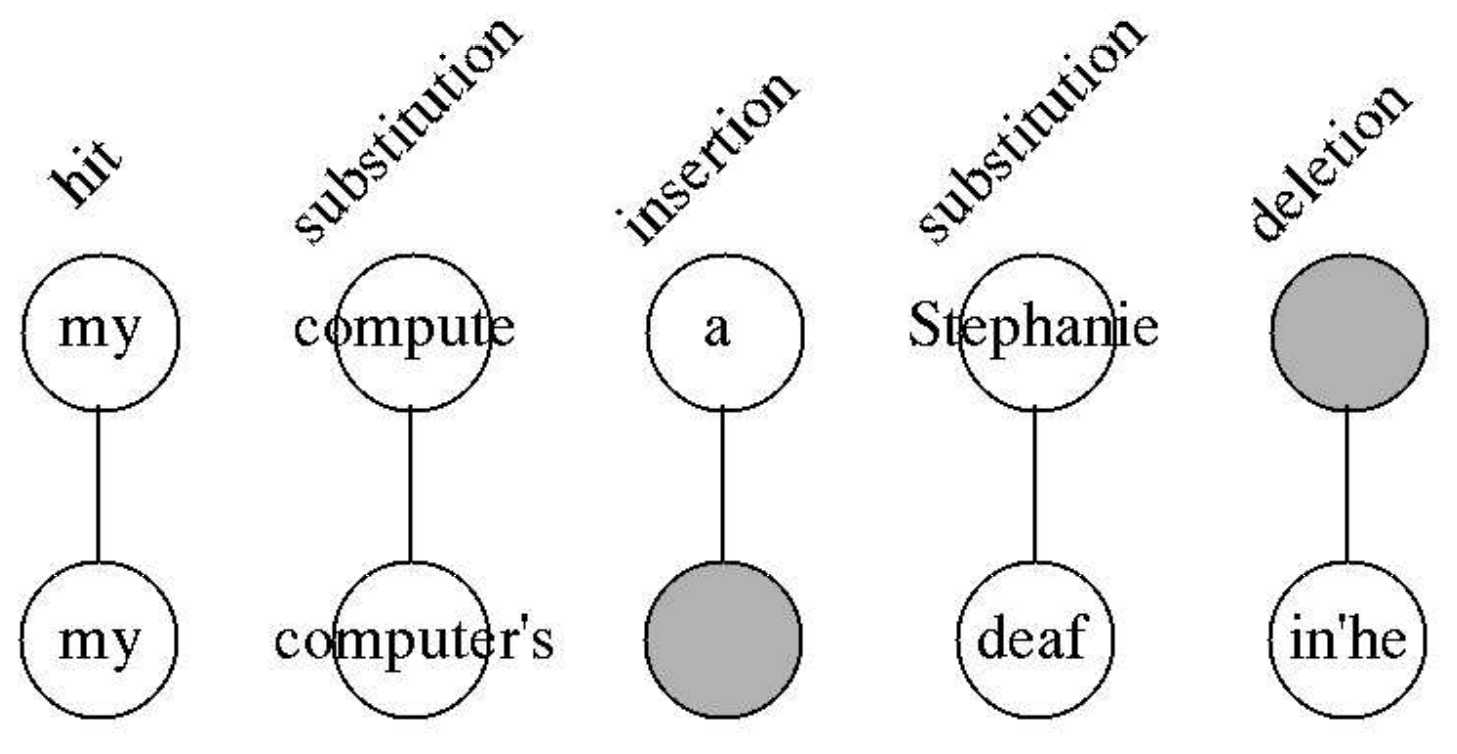
\includegraphics[scale=0.4]{img/wer_letters.png}
		\caption{Example of $H, S, D, I$ classification on the input words “my computer’s deaf in’he?”. From \cite{morris2004and}.}
		\label{fig:wer_letters}
	\end{center}
\end{figure}

\noindent An important aspect is that it is necessary to apply some appropriate pre-processing steps on both the predicted and the ground-truth transcription text. In particular, these operations consists in removing leading and trailing spaces, reducing text to lower case, expanding all contractions and removing punctuation. \\
Finally, it is important to highlight that, while \gls{snr} and \gls{lsd} are calculated on the test set patches, \gls{wer} is calculated on the test set full recordings. 

\section{Results} \label{results}
This section describes and discusses the main results achieved in the reported experiments in order to establish the best model architecture. We provide results on both the Multi-Speaker and the Single-Speaker regimes in order to investigate if the proposed algorithm allows improving the audio \gls{sr} task. \\
Our method is compared to three baselines: a cubic B-spline — which corresponds to the upsampling criteria used in all model pipelines (Figures \ref{fig:tfnet_pipeline}, \ref{fig:tfilm_pipeline}, \ref{fig:proposed_pipeline}) - \gls{tfnet} and \gls{tfilm} Net. \\
We remind that a higher \gls{snr} is better, a lower \gls{lsd} is better and a lower \gls{wer} is better. \\
The results of our experiments over the training set are summarized in tables \ref{tab:s_speaker_tr} and \ref{tab:m_speaker_tr}. As we can see, our solution achieves the best \gls{snr} and \gls{lsd} values on both tasks. However, high training performance are not, in general, always associated with high generalization results. Furthermore, we remind that, in our setting, the training set data distribution is not highly representative of the problem as we filter silence audio frames. \\
Therefore, we use a validation set, which allows to have a more accurate estimate of the generalization power of the models during the training phase. Validation set results can be seen in Table \ref{tab:m_speaker_val}; the proposed model outperforms the other models on \gls{lsd} score, while its \gls{snr} is not as good as the \gls{tfnet} system one. \\

\begin{table}[!htb]
	\begin{center}
		\begin{tabular}{@{}ccccc@{}}
			\toprule
			\multicolumn{5}{c}{\textbf{\begin{tabular}[c]{@{}c@{}}Single-Speaker\\ \textit{\scriptsize{Training Set}}\end{tabular}}}  \\ \midrule
			Obj. & Spline & TFNet & TFiLM Net & Proposed \\ \midrule
			SNR & 14.74 & 16.93 & 16.71 & \textbf{17.33} \\ \midrule
			LSD & 5.64 & 3.44 & 3.93 & \textbf{3.24} \\ \bottomrule
		\end{tabular}
		\caption{Evaluation of \gls{bwe} methods (in \gls{db}) on the Single-Speaker task over the training set in terms of \gls{snr} and \gls{lsd}. A higher \gls{snr} is better and a lower \gls{lsd} is better.}
		\label{tab:s_speaker_tr}
	\end{center}
\end{table}

\begin{table}[!htb]
	\begin{center}
		\begin{tabular}{@{}ccccc@{}}
			\toprule
			\multicolumn{5}{c}{\textbf{\begin{tabular}[c]{@{}c@{}}Multi-Speaker\\ \textit{\scriptsize{Training Set}}\end{tabular}}}  \\ \midrule
			Obj. & Spline & TFNet & TFiLM Net & Proposed \\ \midrule
			SNR & 14.29 & 15.97 & 15.96 & \textbf{16.21} \\ \midrule
			LSD & 6.29 & 3.69 & 4.25 & \textbf{3.37} \\ \bottomrule
		\end{tabular}
		\caption{Evaluation of \gls{bwe} methods (in \gls{db}) on the Multi-Speaker task over the training set in terms of \gls{snr} and \gls{lsd}. A higher \gls{snr} is better and a lower \gls{lsd} is better.}
		\label{tab:m_speaker_tr}
	\end{center}
\end{table}

\begin{table}[!htb]
	\begin{center}
		\begin{tabular}{@{}ccccc@{}}
			\toprule
			\multicolumn{5}{c}{\textbf{\begin{tabular}[c]{@{}c@{}}Multi-Speaker\\ \textit{\scriptsize{Validation Set}}\end{tabular}}}  \\ \midrule
			Obj. & Spline & TFNet & TFiLM Net & Proposed \\ \midrule
			SNR & 13.60 & \textbf{15.57} & 15.35 & 15.34 \\ \midrule
			LSD & 5.97 & 3.57 & 4.14 & \textbf{3.31} \\ \bottomrule
		\end{tabular}
		\caption{Evaluation of \gls{bwe} methods (in \gls{db}) on the Multi-Speaker task over the validation set in terms of \gls{snr} and \gls{lsd}. A higher \gls{snr} is better and a lower \gls{lsd} is better.}
		\label{tab:m_speaker_val}
	\end{center}
\end{table}

\noindent At this point, we can examine the extent to which the models generalize across the test set. The results of \gls{snr} in Figure \ref{fig:snr} show that \gls{tfnet} approach is the one which achieves the best values on both tasks. As for the other two methods, they achieve similar performance. Furthermore, we can observe that each model exceeds the spline baseline about more than 1\gls{db}. \\
As for \gls{lsd} scores, we can see from Figure \ref{fig:lsd} that our system shows an improvement of 0.1 - 2.2 \gls{db} over the baseline methods on the Single-Speaker task and even of 0.3 - 2.3 \gls{db} on the Multi-Speaker problem. From an intuitive perspective, we can say that, in our model, the spectral distortions of the predicted speech from the clean speech is less significant at high-frequencies. \\
These two metrics reflect the potential of the models to help the Deep Speech engine in better performing the \gls{stt} conversion. In fact, as we can see from Figure \ref{fig:wer}, the results of \gls{wer} show that the two best models are again \gls{tfnet} and the proposed one. In particular, we can see that our approach outperforms by approximately 0.05 percentage points the \gls{tfnet} system, by $\approx$ 0.08 percentage points the \gls{tfilm} Net and by $\approx$ 0.12 percentage points the spline baseline. Although these results are quite far from the \gls{wer} obtained on original recordings (which is an estimate of the real potential of the Deep Speech engine), the improvements brought by the audio \gls{sr} models are remarkable when compared to splines.\\
\begin{figure}[H]
	\begin{center}
		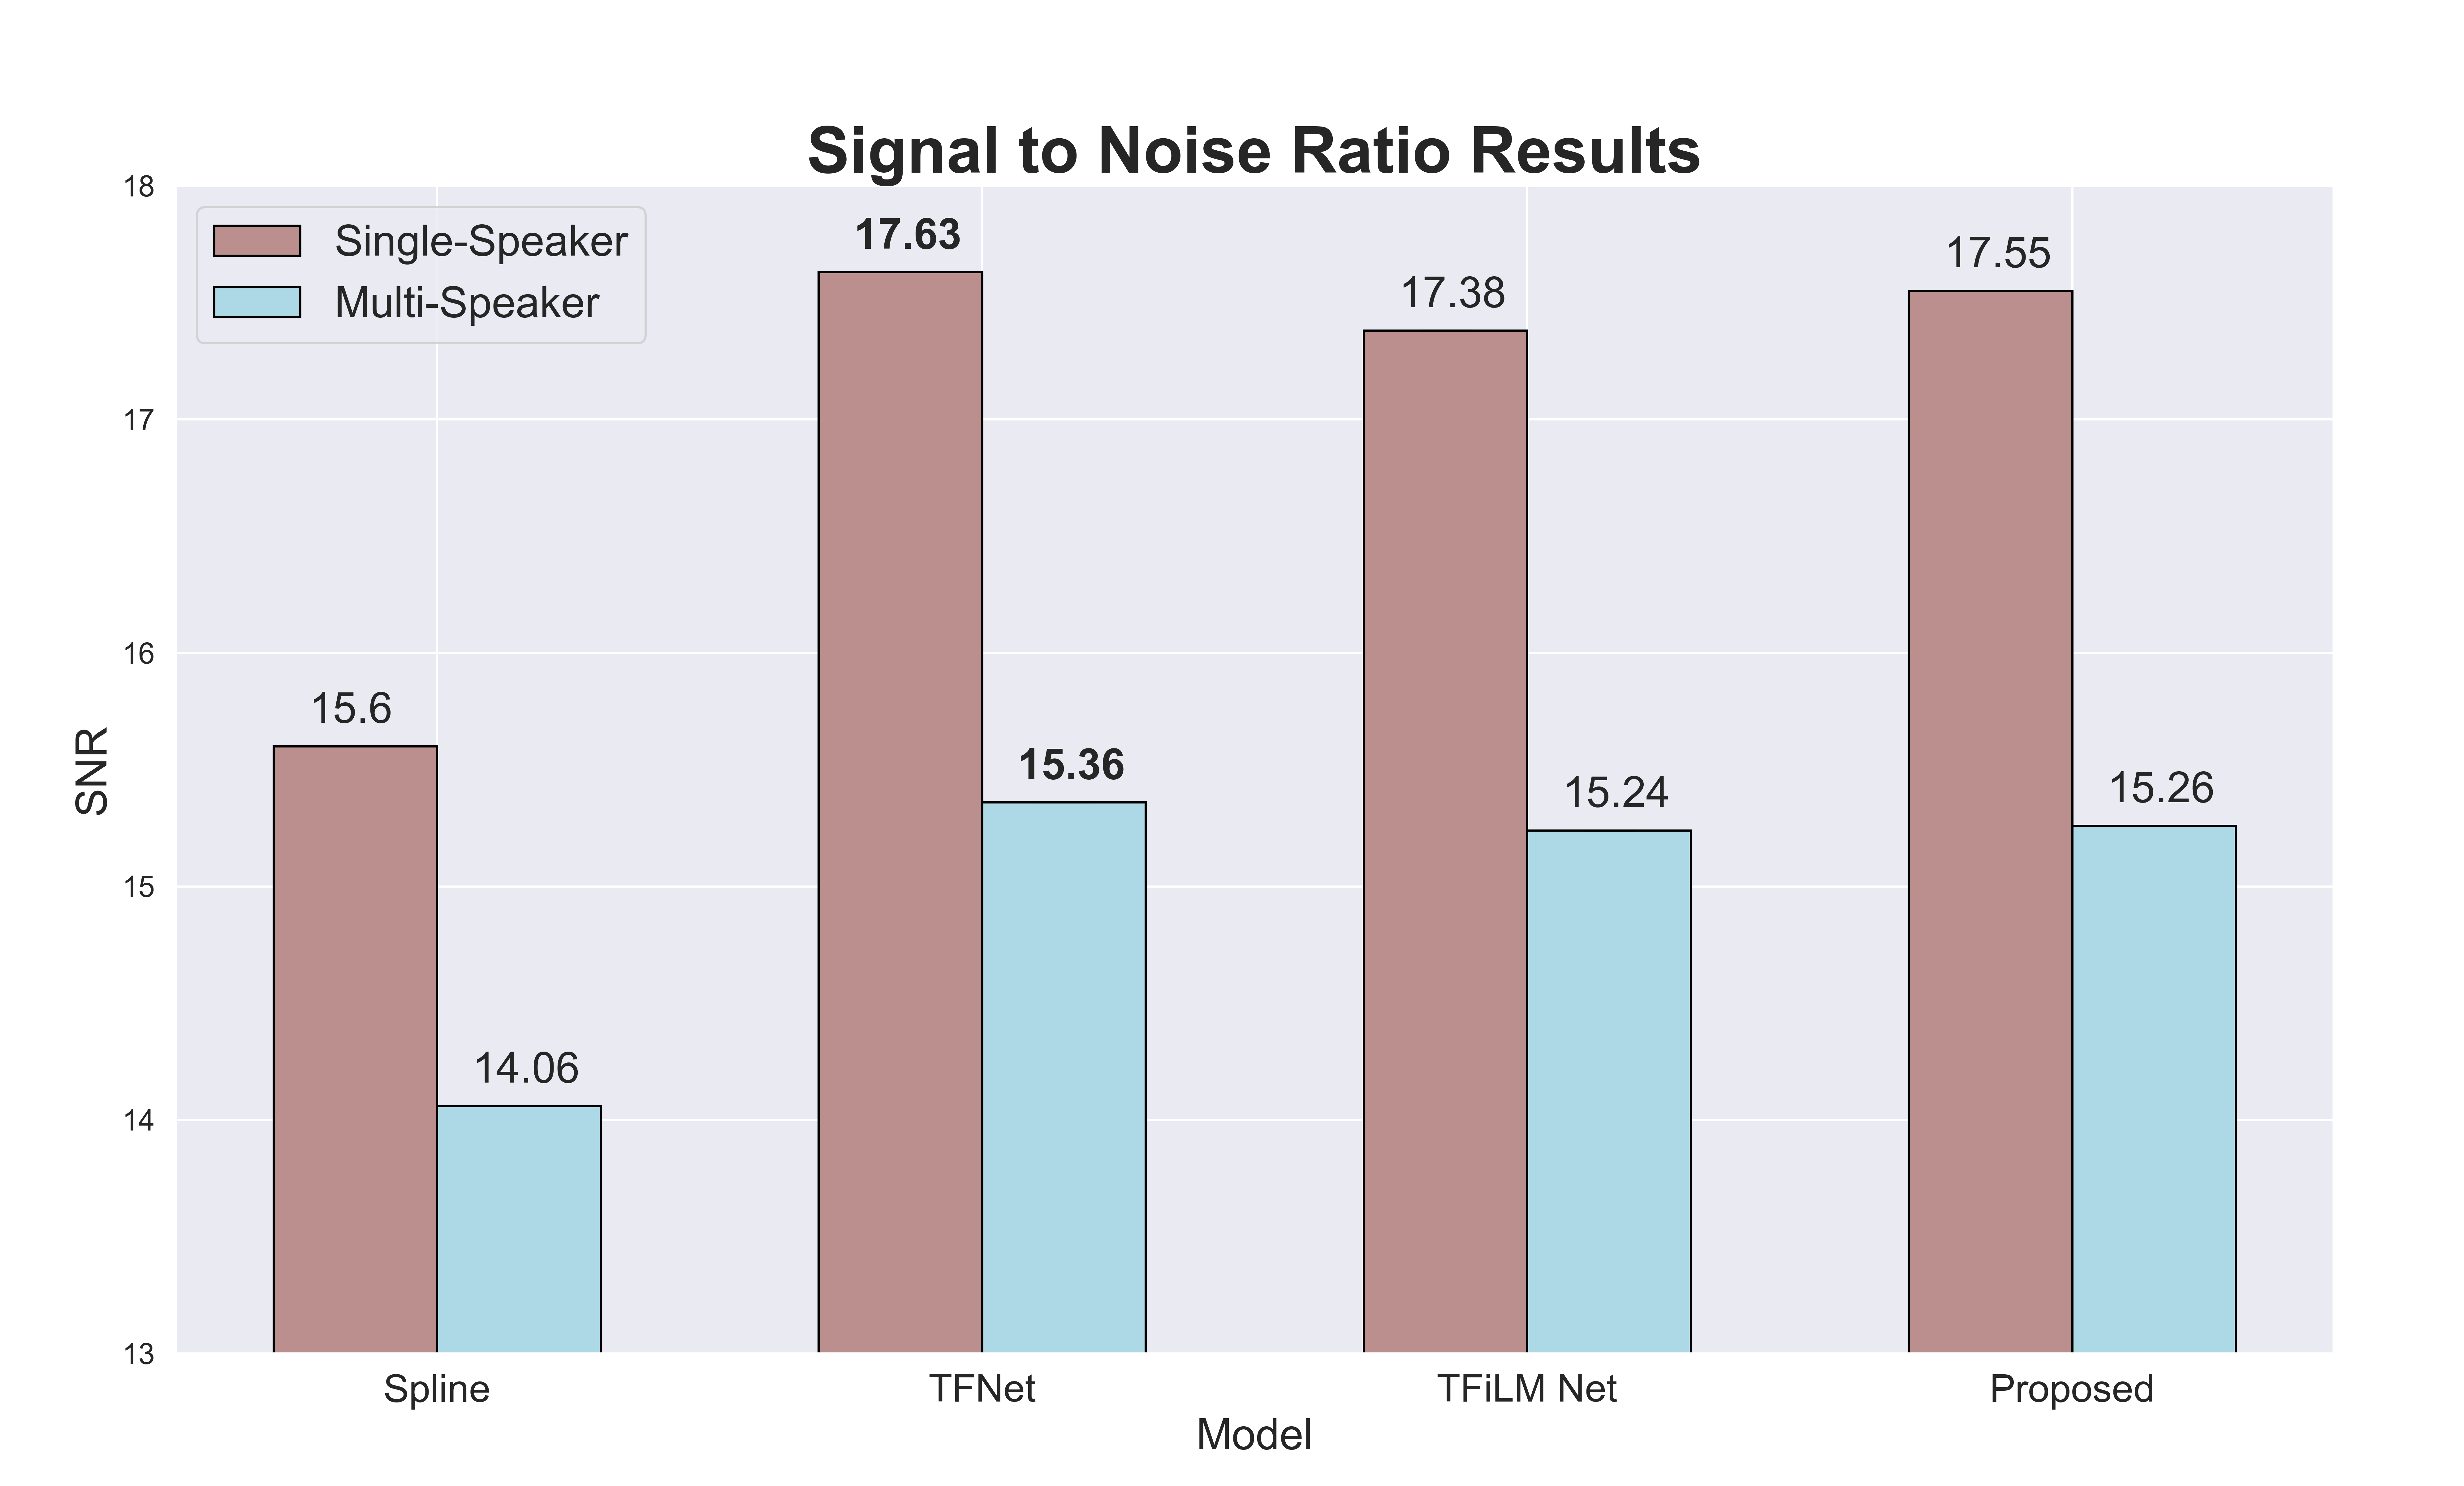
\includegraphics[scale=0.4]{img/snr_results.png}
		\caption{SNR results (in \gls{db}) on Test Set for both Single-Speaker and Multi-Speaker tasks. Higher is better.}
		\label{fig:snr}
	\end{center}
\end{figure}

\begin{figure}[!htb]
	\begin{center}
		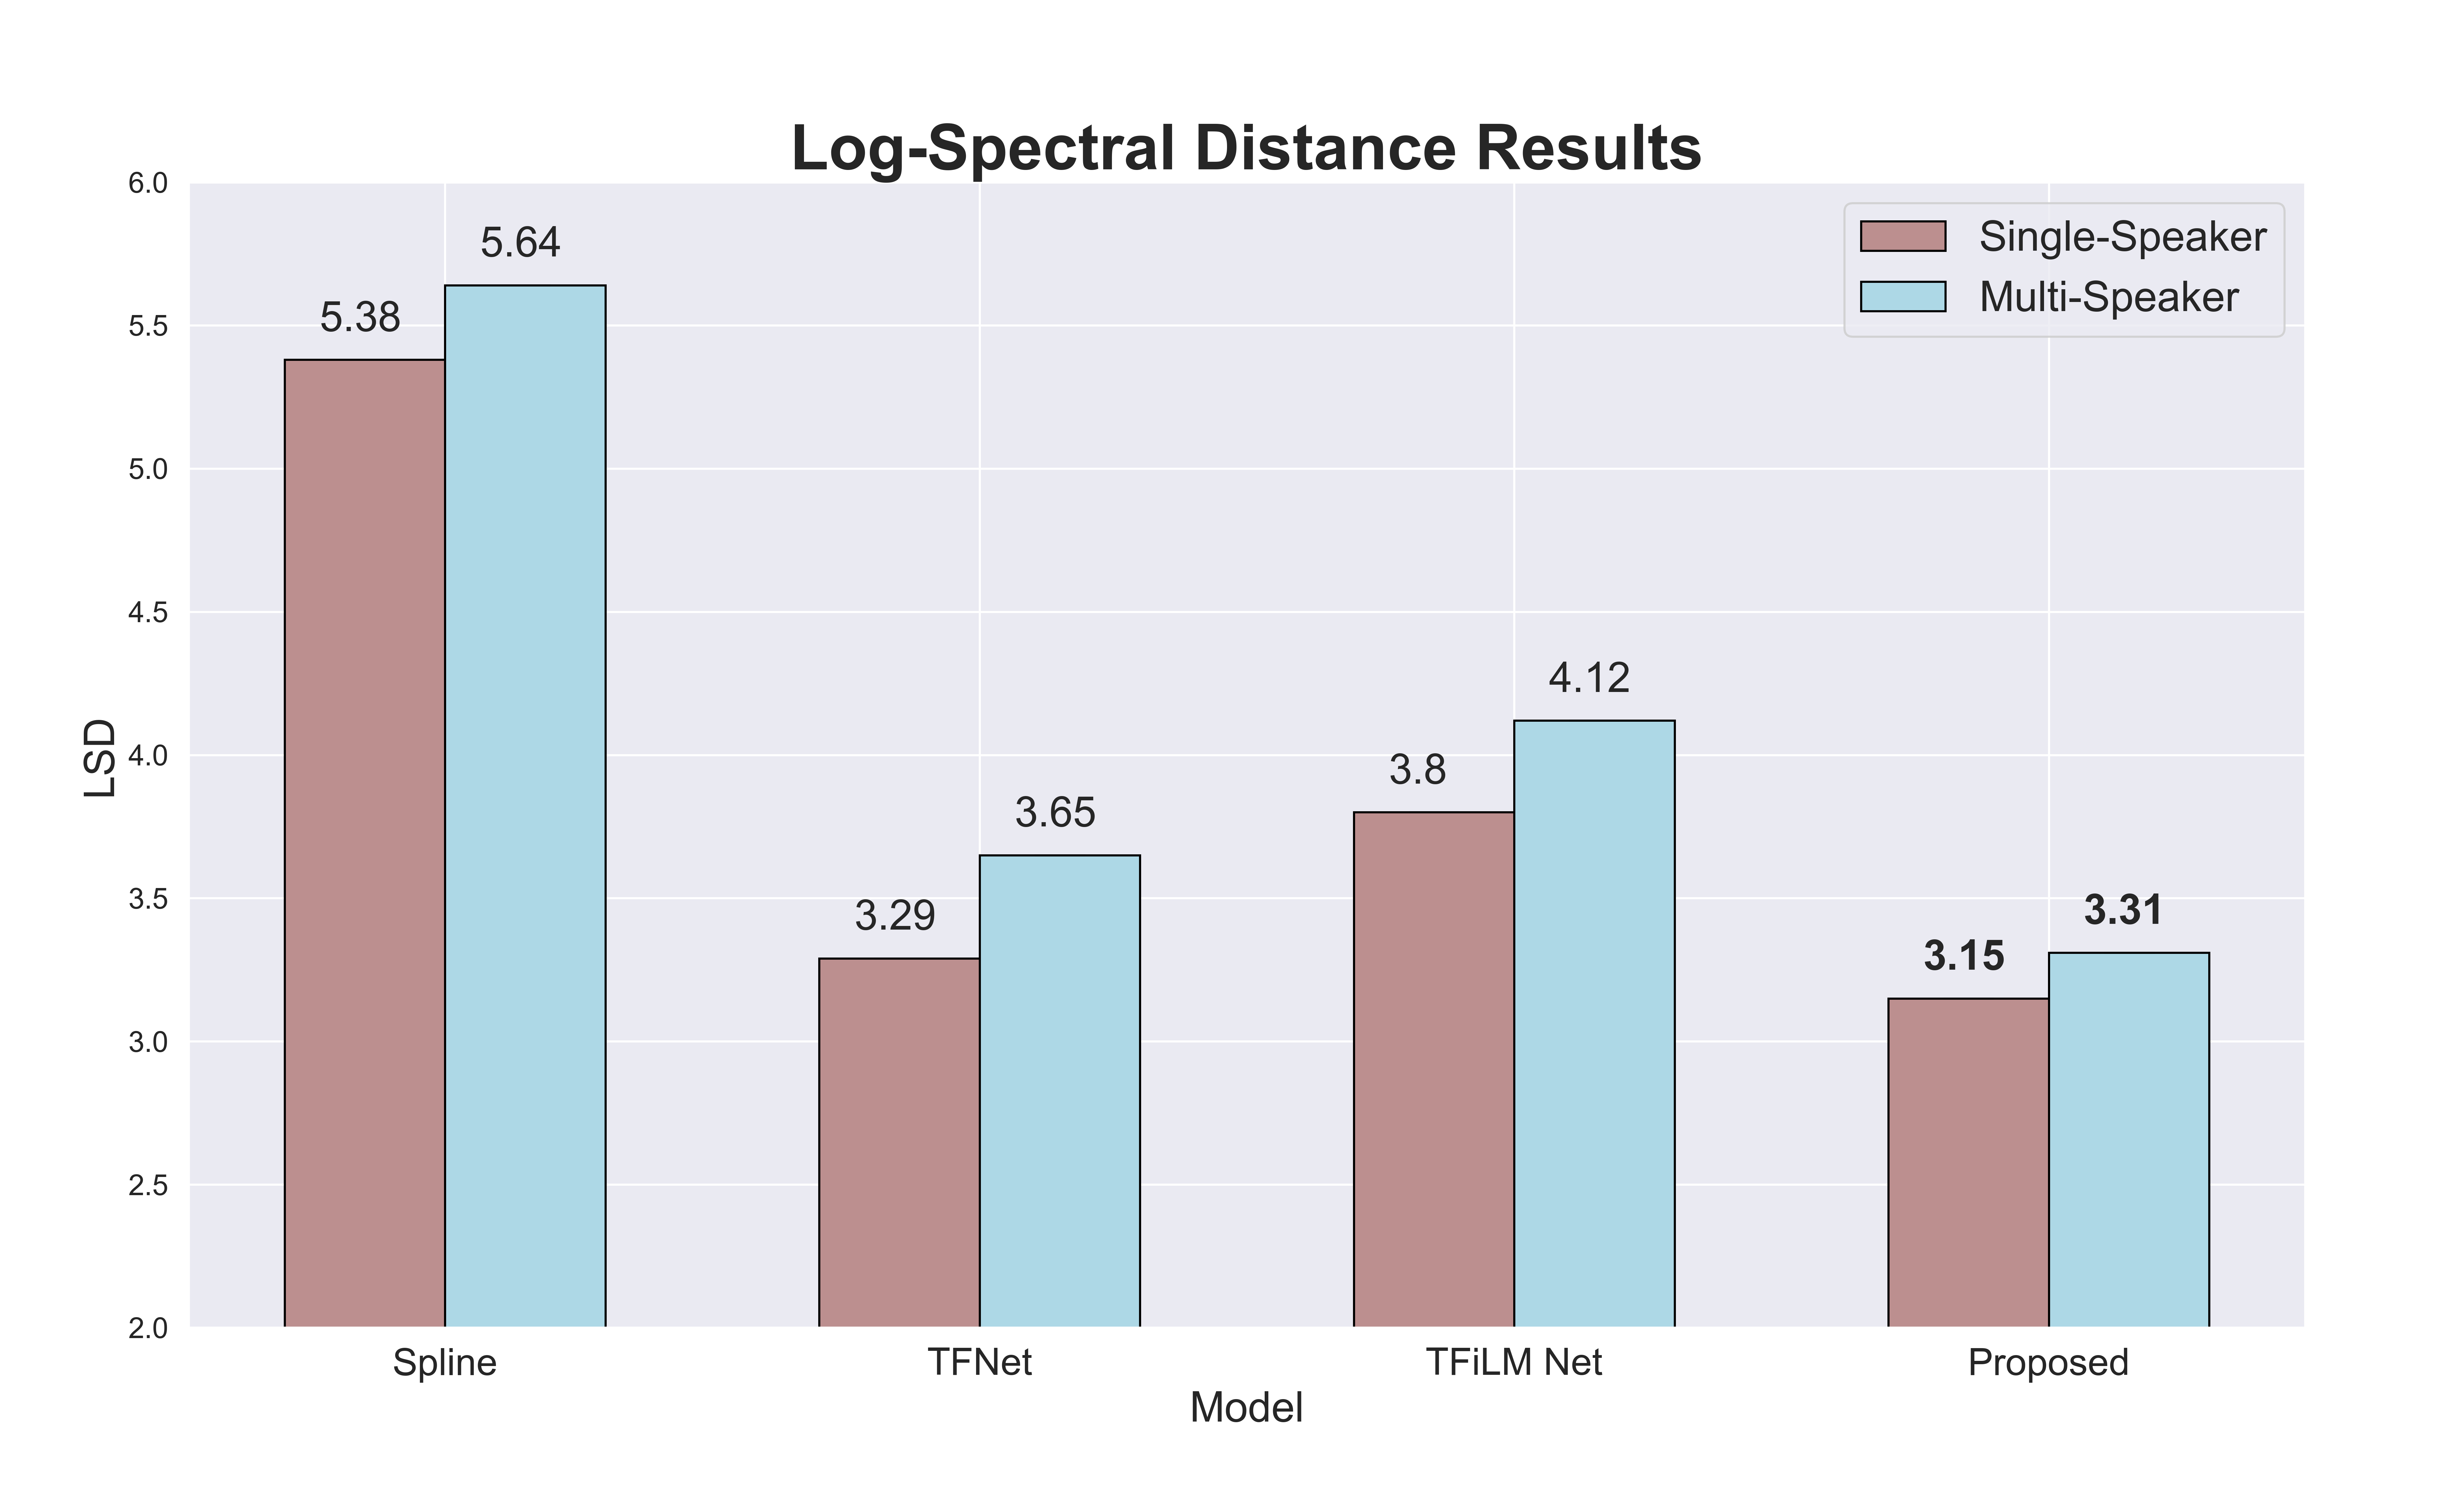
\includegraphics[scale=0.4]{img/lsd_results.png}
		\caption{LSD results (in \gls{db}) on Test Set for both Single-Speaker and Multi-Speaker tasks. Lower is better.}
		\label{fig:lsd}
	\end{center}
\end{figure}

\begin{figure}[!htb]
	\begin{center}
		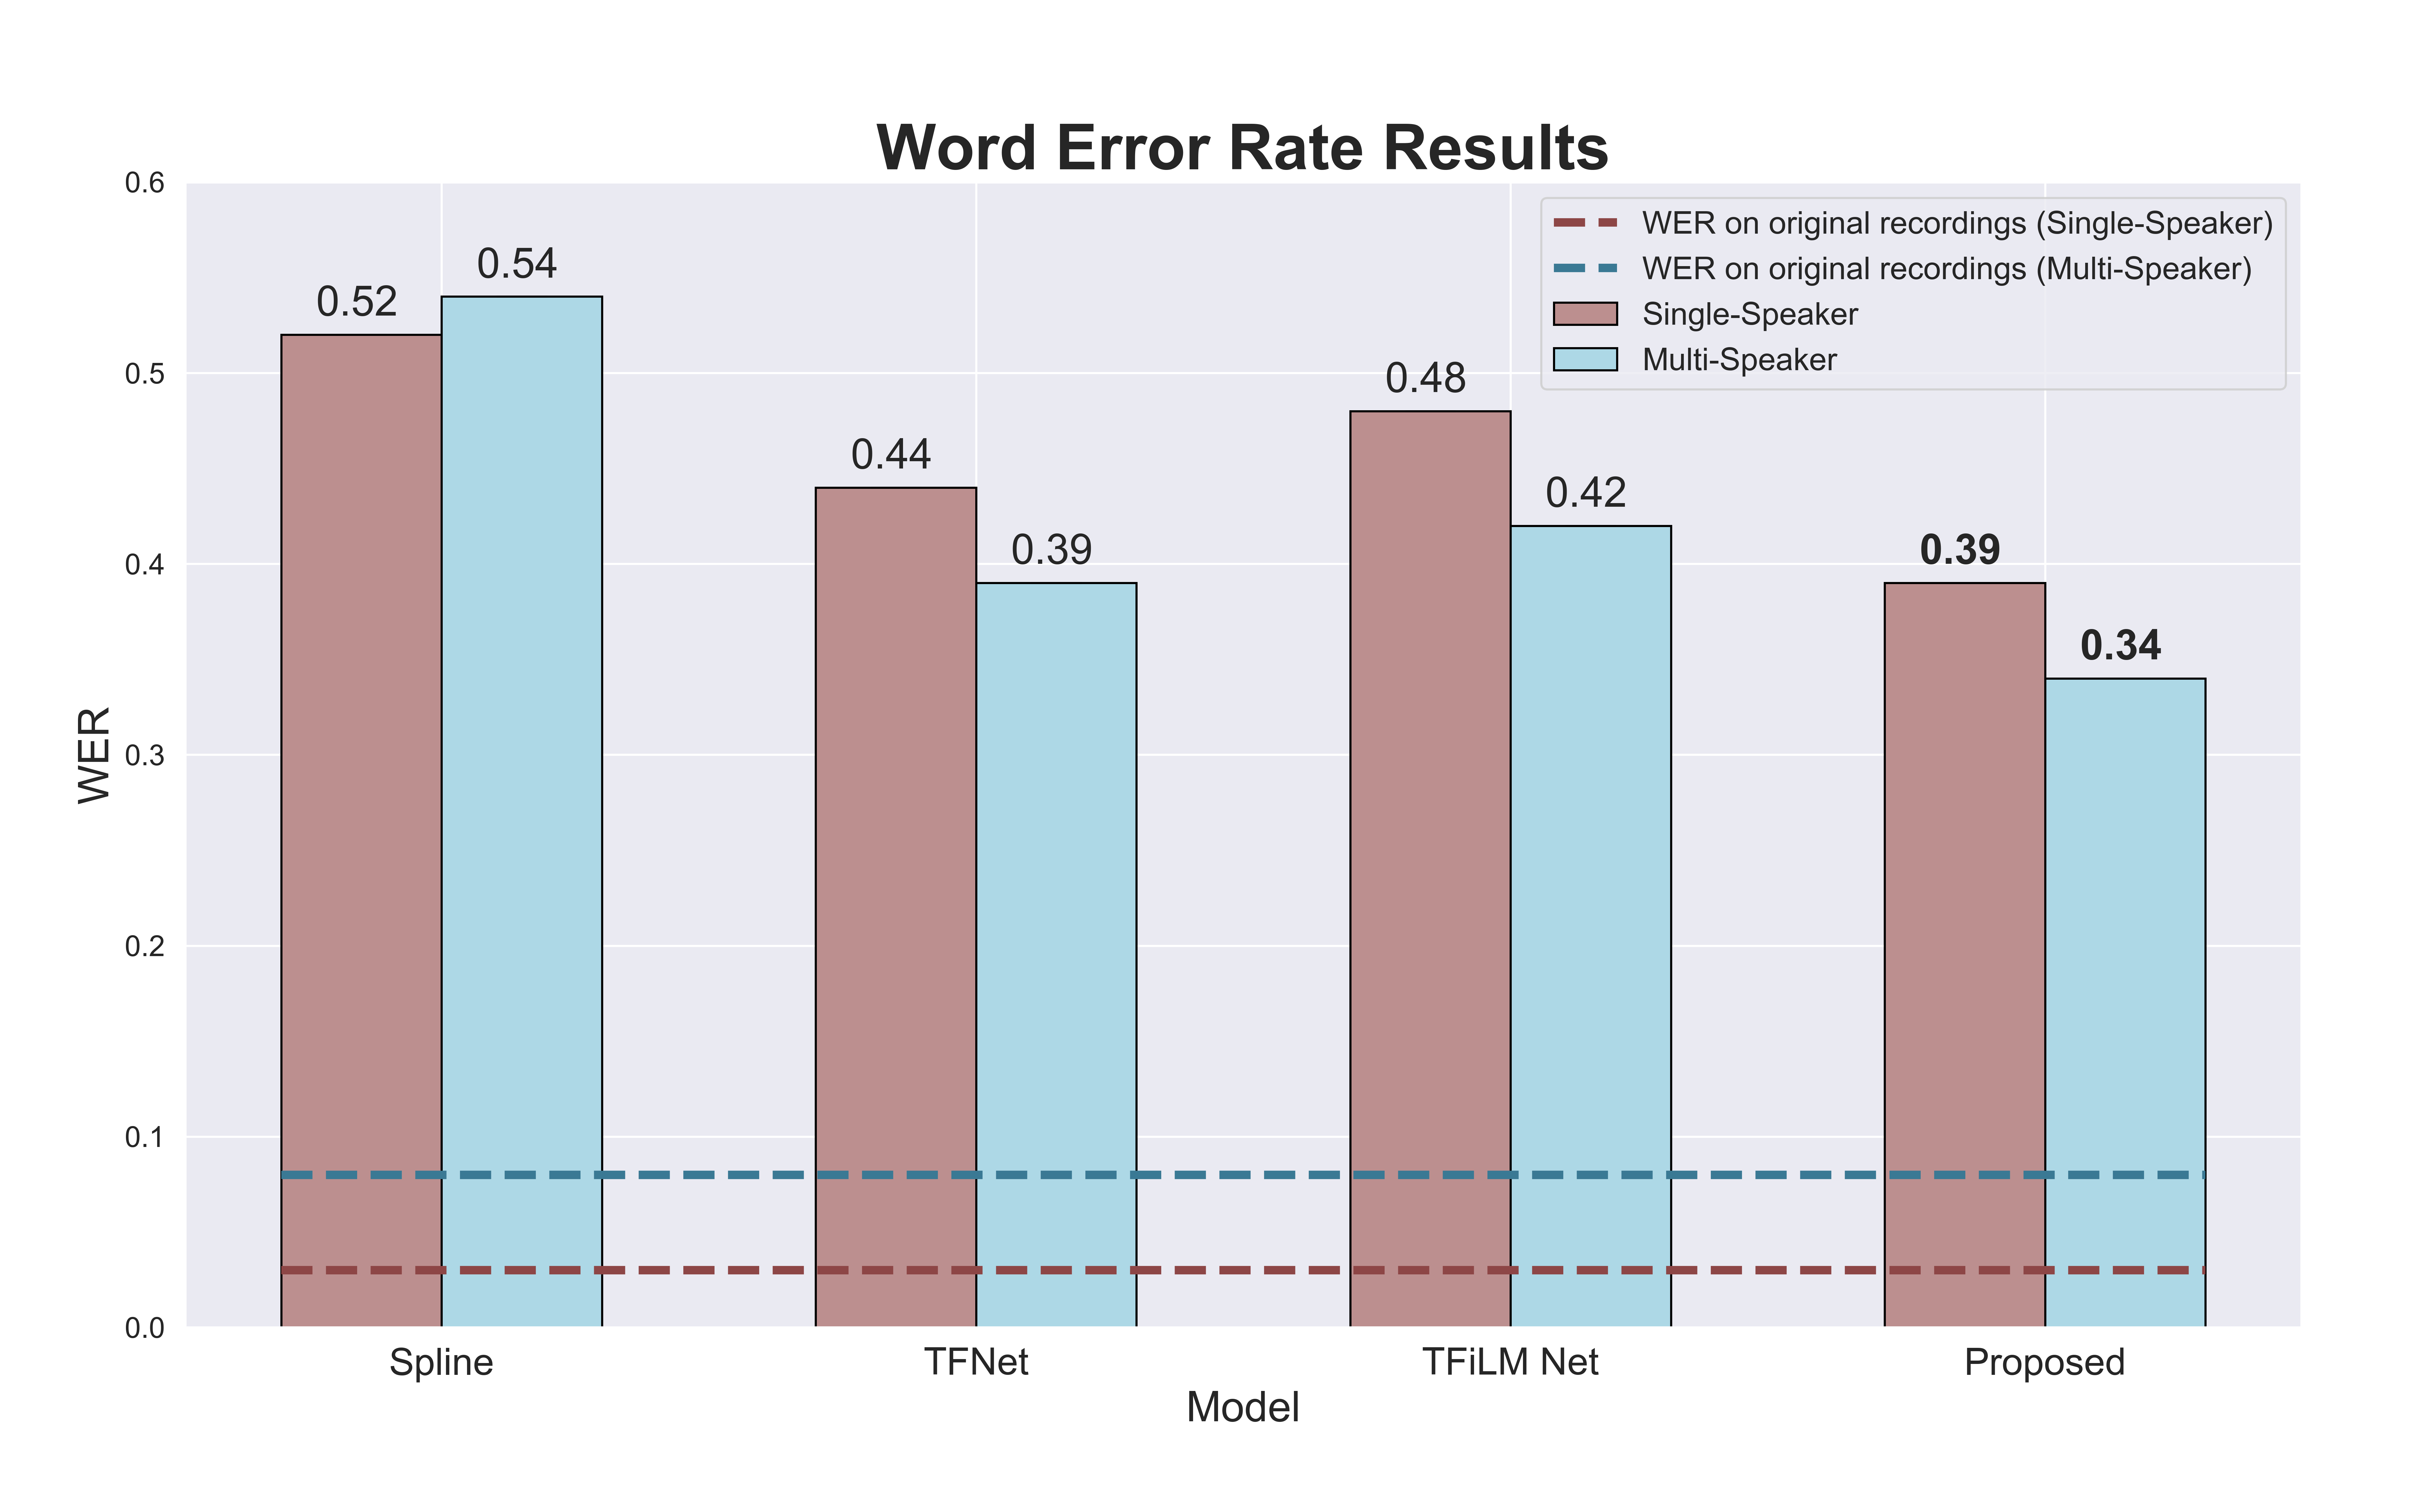
\includegraphics[scale=0.4]{img/wer_results.png}
		\caption{\gls{wer} results (in percentage) on Test Set for both Single-Speaker and Multi-Speaker tasks. \gls{wer} on original recordings is, respectively, equal to 0.03 and 0.08. Lower is better.}
		\label{fig:wer}
	\end{center}
\end{figure}

\noindent Therefore, it is fair to say that the proposed approach and the \gls{tfnet} system are the best model according to these quantitative metrics. There is not a clear winner, since the best model changes according to the considered metric. Thus, although \gls{tfnet} achieves the best \gls{snr}, the proposed model shows a better reconstruction quality in the frequency domain. Furthermore, our approach is the one which better helps the Deep Speech engine in converting audio data to text. This latter result is in agreement with the \gls{lsd} metric evaluation, and suggests that the proposed method provides a better speech quality. \\
Finally, it is worth observing the audio spectrograms. They show ~-~ from up to down in figures \ref{fig:original_signal_spec} \ref{fig:lowres_signal_spec}, \ref{fig:model_signal_spec} ~-~ a high-resolution signal, its low-resolution version obtained using spline interpolation, and the output of our model. These examples refer to an audio file that belong to the test set of the Multi-Speaker task (speaker ID and audio file ID are, respectively, \textit{p351} and \textit{004}).\\
It is important to mention that these spectrograms are computed using consecutive Fourier transforms; in particular, we use a \textit{Hamming} window of 512 samples with 50\% overlap.\\
As we can see, the proposed model is generally able to reconstruct a remarkable part of the original signal’s spectral content, especially in the frequency range 2 - 4 k\gls{hz}. It is worth noting that its estimation is mainly focused on the speech frames rather than the silence ones and this makes perfect sense. 

\begin{figure}[!htb]
	\begin{center}
		\includegraphics[scale=0.5]{img/original_signal_spec.png}
		\caption{Spectrogram showing how the frequency content of a 16kHz signal changes over time.}
		\label{fig:original_signal_spec}
	\end{center}
\end{figure}

\begin{figure}[!htb]
	\begin{center}
		\includegraphics[scale=0.5]{img/lowres_signal_spec.png}
		\caption{Spectrogram showing the spline reconstruction of the signal.}
		\label{fig:lowres_signal_spec}
	\end{center}
\end{figure}

\begin{figure}[!htb]
	\begin{center}
		\includegraphics[scale=0.5]{img/model_signal_spec.png}
		\caption{Spectrogram showing the model reconstruction of the signal.}
		\label{fig:model_signal_spec}
	\end{center}
\end{figure}

\subsubsection{Spectral Fusion Layer Weights Analysis}
We perform an additional analysis on the weights $w$ introduced in the Spectral Fusion Layer (see Equation \ref{eq:spectralfusion1}). In particular, we remind that $w$ is a trainable vector which establish the weight of each branch for the spectral magnitude prediction; the higher its values are, the more the weight of the time branch is important in the spectral magnitude $M$ calculation. Our goal is to investigate how these weights are distributed on both the proposed model and the \gls{tfnet} system.\\
This analysis is only performed for the Multi-Speaker task; however, it is reasonable to assume that the results are not very different in the Single-Speaker task since the models are trained using a fine-tuning approach. \\
The resulted distribution for both the proposed and the \gls{tfnet} models is provided in Figure \ref{fig:weights_results}. \\
\begin{figure}[H]
	\begin{center}
		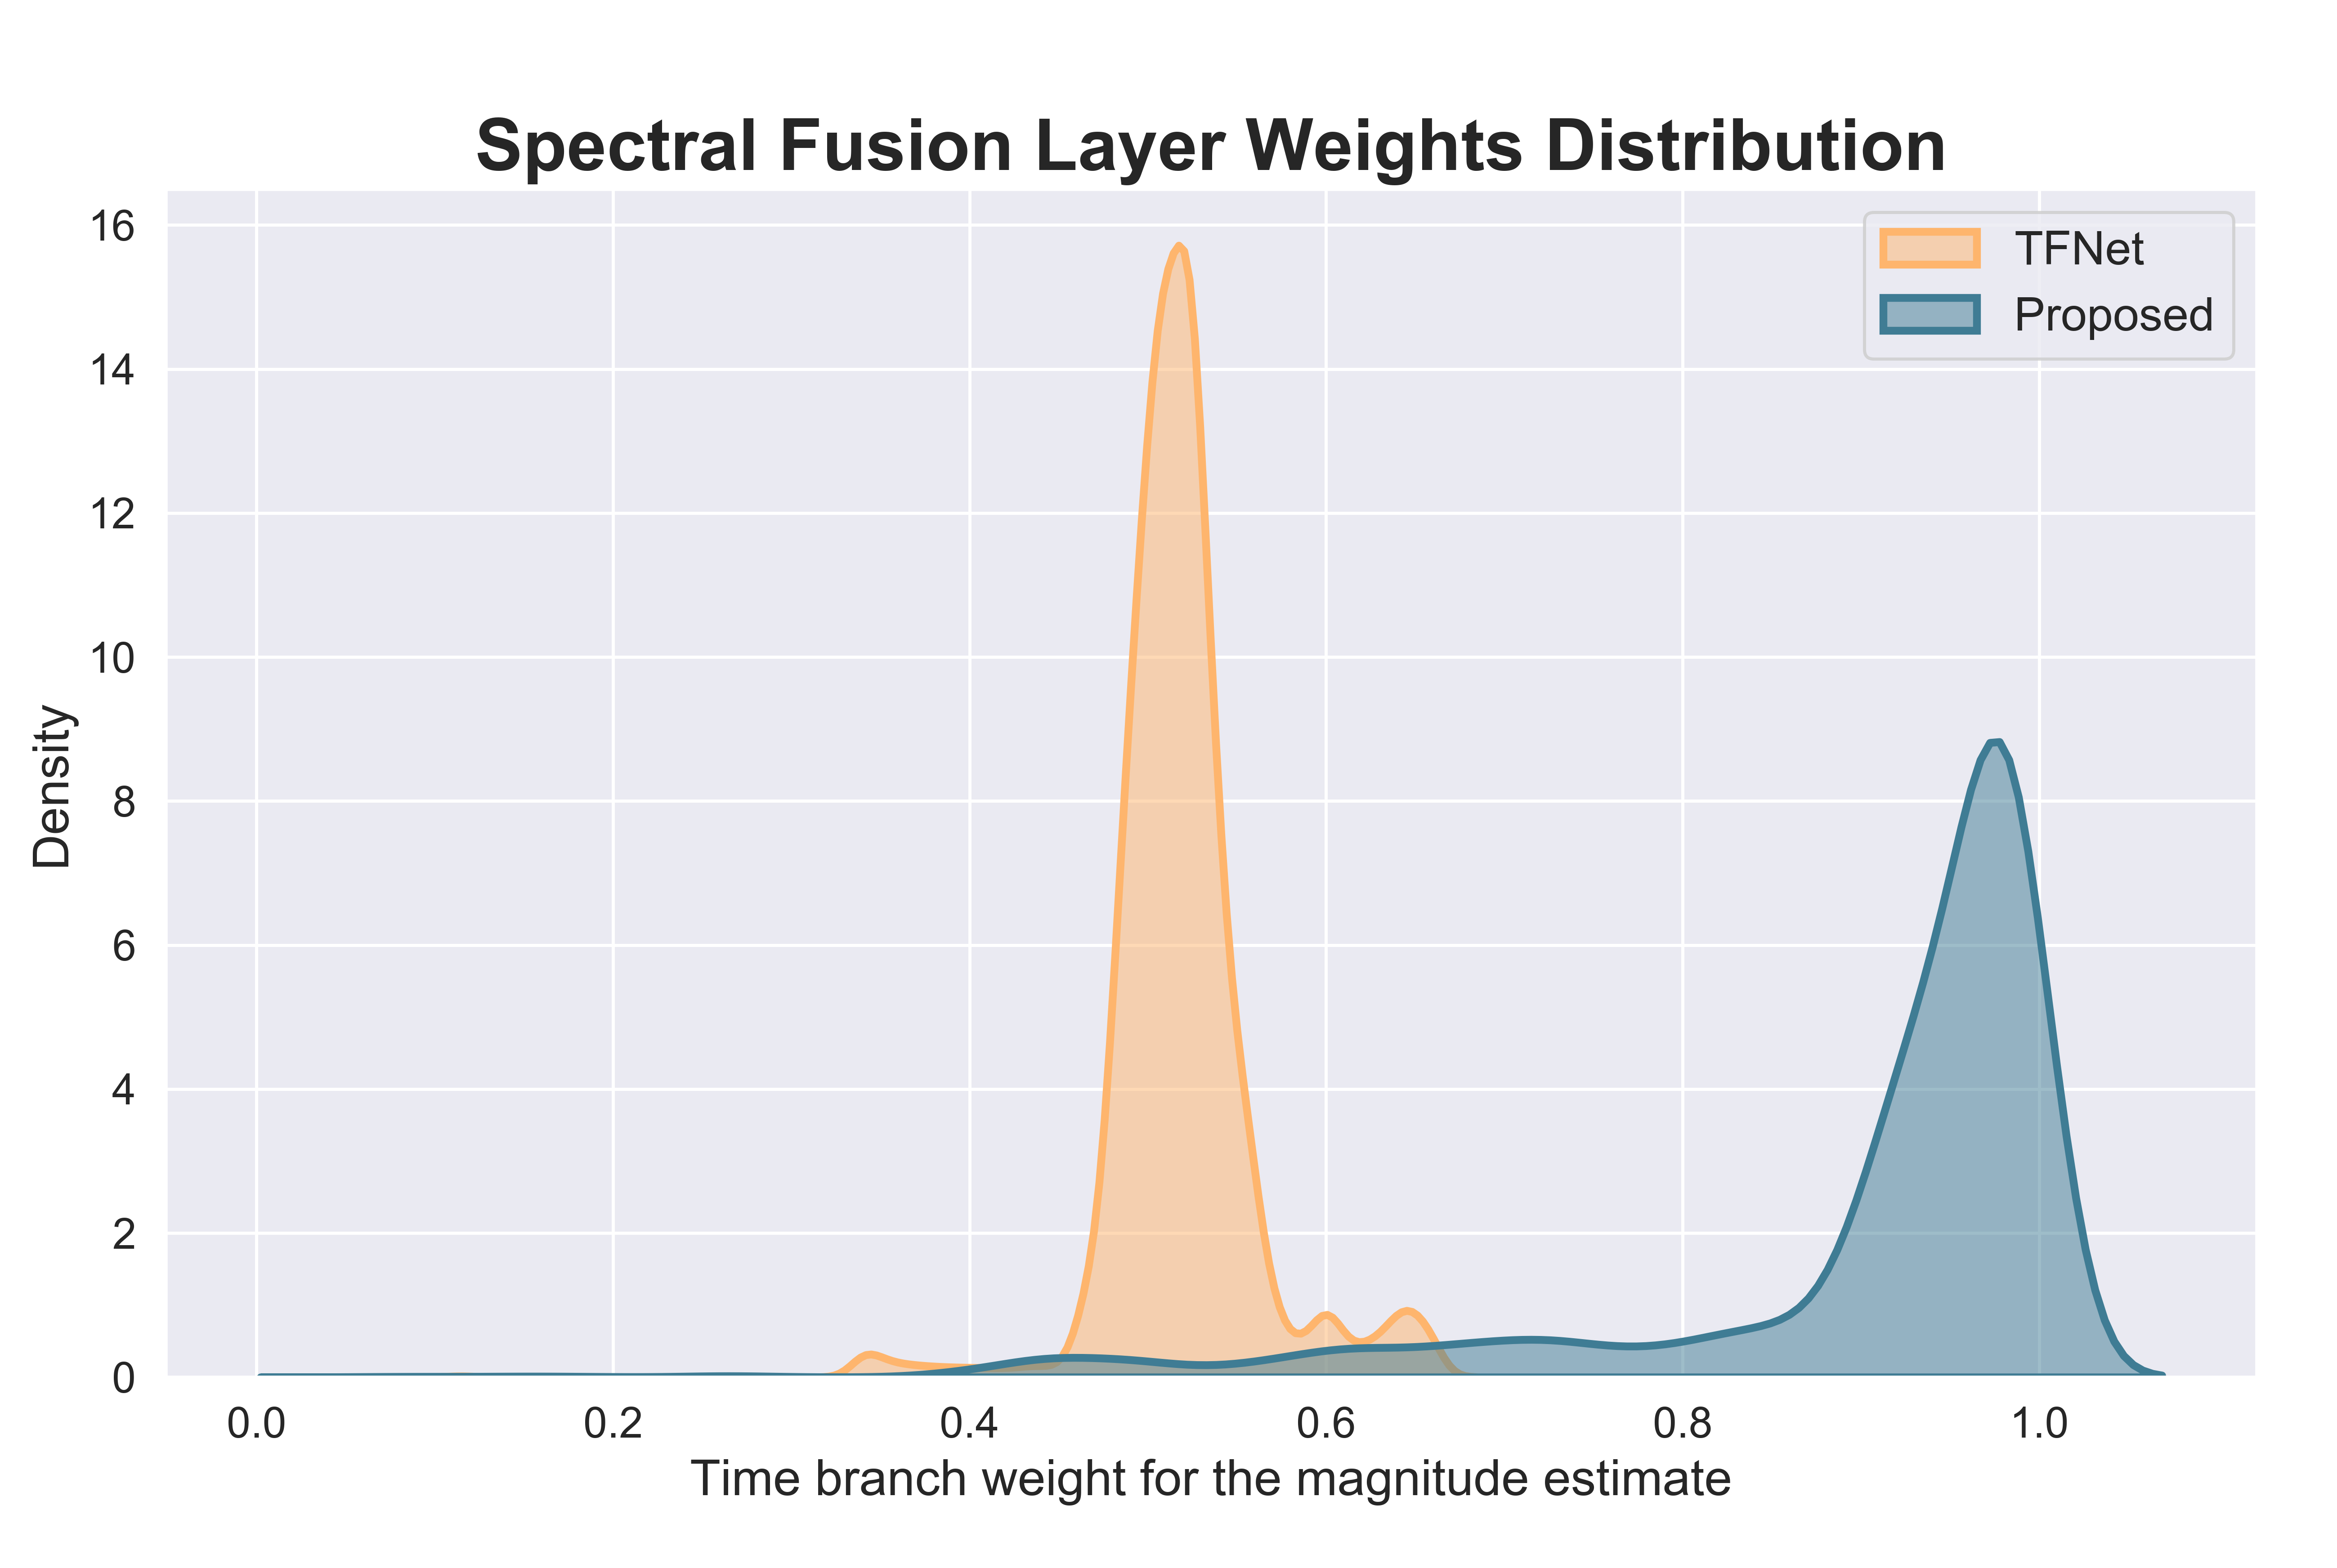
\includegraphics[scale=0.62]{img/weights_results.png}
		\caption{Spectral Fusion Layer weights distribution for both the \gls{tfnet} model and the proposed system.}
		\label{fig:weights_results}
	\end{center}
\end{figure}
\noindent As we can see, the weights of the two branches are more balanced in the \gls{tfnet} system than in the proposed model. In fact, the two means are, respectively, $\widebar{w}_{TFNet} \approx 0.5$ and  $\widebar{w}_{Proposed} \approx 0.9$. \\
Consequently, it is fair to say that, on average, for the \gls{tfnet} system the two branches contributes equally to the spectral magnitude $M$ estimation. On the other hand, for our model the two branches contribution is heavily skewed. \\
Although we cannot prove it mathematically, it is reasonable to think that this is a limitation for our model. In fact, the spectral branch, whose only goal is to contribute to the estimate of $M$, turns out not to be relevant in the final prediction. In other words, since the phase estimation is strictly time-branch dependent, the spectral branch in our model results to be almost irrelevant for the \gls{hr} reconstruction. \\
